% !TEX root = ../thesis-example.tex

\chapter{History and State of the Art} \label{sec:bg}
Computing is at one of its most exciting moments in history, playing an essential role in supporting many important human activities. The explosion in the availability of information in different media forms and through multiple sensors and devices means, on one hand, that the amount of data we can collect will continue to increase dramatically, and, on the other hand, that we need to develop new paradigms to search, organize, and integrate such information to support all human activities.
Human-centered computing (HCC) is a set of methodologies that apply to any field that uses computers, in any form, in applications in which human directly interact with systems or information that use computer technologies \cite{Jaimes2006f}.
\add{HCC is an emerging field that aims at tightly integrating human sciences and computer sciences for timely cognitive and interactive support.}
It focuses on humans from beginning to end. HCC also aims at radically changing computing with new methodologies to design and build systems that support and enrich people's lives. 

Perception and interaction are the communication between user and computer and important parts of HCC. On the user-side, communication is in task-language and on the system side, in core language. 
In this chapter we want to provide the reader with the necessary and relevant background information about perception and interaction with medical information during procedures, such as medical education, rehabilitation exercise, and intra-oprative interaction.
Then we will turn our attention to topics that are related to mixed reality and natural user interface using gestures. 

\section{Perception and interaction with medical information}
Different medical knowledge is collected through many years of practice and different imaging methodologies, and the knowledge has to be transferred to fresh medical students through medical education and the general population through public education. 
Additionally, during surgery and for each patient, quite a lot of information is collected for diagnosis and navigation.
%, the surgeon has to perform interaction with this information during the operation. 
Good communication between the patient and the surgeon is also very important for making the patient comply with the treatment. 
Rehabilitation exercises also have to be performed after surgery, if need be.
During the above-mentioned procedure, people act different roles to perceive and interact with medical information. In this section, we discuss the states and challenges for the perception and interaction with medical information in medical education, public and patient education, rehabilitation exercise and in operating rooms.

\subsection{Medical education}
While medical education has already performed for a long time, we start from Abraham Flexner's report in 1910 \citep{Flexner1910}. Flexner visited all 155 medical schools that existed in North America in 1909 and he identified four major problems of medical education: lack of standardization, lack of integration, lack of inquiry, and identity formation. The report had a huge impact and shaped modern medical education, where patient care, teaching, and research are combined. However, academic hospitals don't spend enough time on teaching today due to enormous pressure to publish and for economic reasons \cite{Saidi2007}. Another problem is that today the research is focusing on very small subtopics, which do not relate to medical education \cite{Ludmerer2003}. On the other hand, only a little research is done for teaching. An example is gross anatomy where most topics are already know and only very few interesting research exists.
In today's medical schools students are required to understand both function and spatial context of human anatomy. 

\subsubsection{Traditional methodologies} 
Traditional medical education learning is classified into three categories: cadaver, model, and book-based. Although technology has advanced significantly in the last decades, classical school education still mostly uses the same methods to convey anatomical knowledge \cite{Dunnill2013}. Typically, the information is collected in printed books like anatomy atlases, displayed in the form of charts and diagrams. Those diagrams provide a simple and well-known method to illustrate form and appearance of organs, having the advantage that the user is accustomed to such methods of display. However, there exist several downsides to this method. First of all, the view is limited to a selected few different angles the author chose to present. This may not be sufficient in some cases to fully convey how an organ is situated relative to its surroundings since occlusions limit the possibilities to visualize these spatial relations \cite{AGilroyBMacpherson2012}. Another problem is that often the organs are only depicted schematically by leaving out details or distorting tissue colors, thus giving only a coarse impression on how the organ actually looks like in reality.
For example, it is difficult to interpret the spatial and physical characteristics of anatomy by observing two-dimensional images, diagrams, or photographs. Many physical models also lack detail levels to fully understand the specific anatomy (see \figurename{\ref{fig:2-bg:traditionalMethods}}). 
\begin{figure}
	\centering
	\subfloat[Atlas.]{\includegraphics[height=0.4\linewidth]{figures/2-bg/atlas}}
	%\qquad
	\subfloat[Physical model.]{\includegraphics[height=0.4\linewidth]{figures/2-bg/models}}
	\caption{Traditional methodologies for Medical learning.}
	\label{fig:2-bg:traditionalMethods}
\end{figure}

Anatomy education is also performed by the dissection of cadavers.  The value of dissection classes as a teaching format lies in the fact that it provides a 3D view on human anatomy including tactile learning experiences. It enables elaboration of knowledge already acquired in lectures and study books and it provides an overall perspective of anatomical structures and their mutual relations in a whole organism \cite{McLachlan2004}. 
The cadaver-based learning has seen decline due to practical and cost issues (see \figurename{\ref{fig:2-bg:cadaver}}). And so far, no objective empirical evidence exists concerning the effectiveness of dissection classes for learning anatomy \cite{Frank2005}.
\begin{figure}
	\centering
	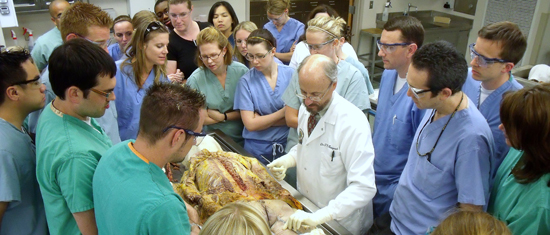
\includegraphics[width=0.8\linewidth]{figures/2-bg/cadaver}
	\caption{Anatomy learning with cadaver. It is a very important training but too expensive, and there are always a lot students around one cadaver.}
	\label{fig:2-bg:cadaver}
\end{figure}

\subsubsection{Computer-based learning material} 
It is developed by experts and students can use these materials if there is no available expert in the hospital. Computer-based education can be very powerful for anatomy teaching, where 3D visualization is of great benefit (see \figurename{\ref{fig:2-bg:zygote-body-esplorazione}}). Many virtual model databases exist and E-learning is commonly used today. These resources are very valuable and are more interactive and interesting than textbooks. 
In addition, the personalization in E-learning systems has been the subject of much recent research and allows teachers to select parameters and combine them flexibly to define different personalized strategies according to the specifics of the courses. In recent times, more and more digital methods evolve which are trying to improve on these methods. 
\begin{figure}
\centering
\subfloat{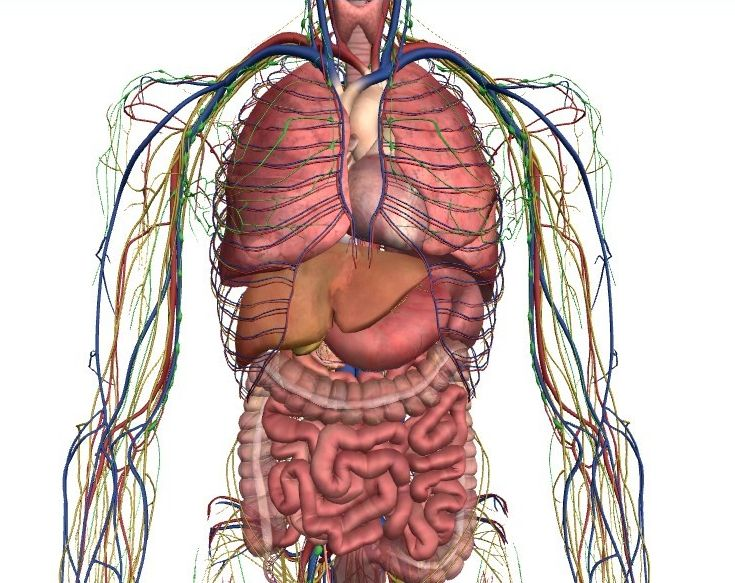
\includegraphics[height=0.4\linewidth]{figures/2-bg/zygote-body-esplorazione}}
\qquad
\subfloat{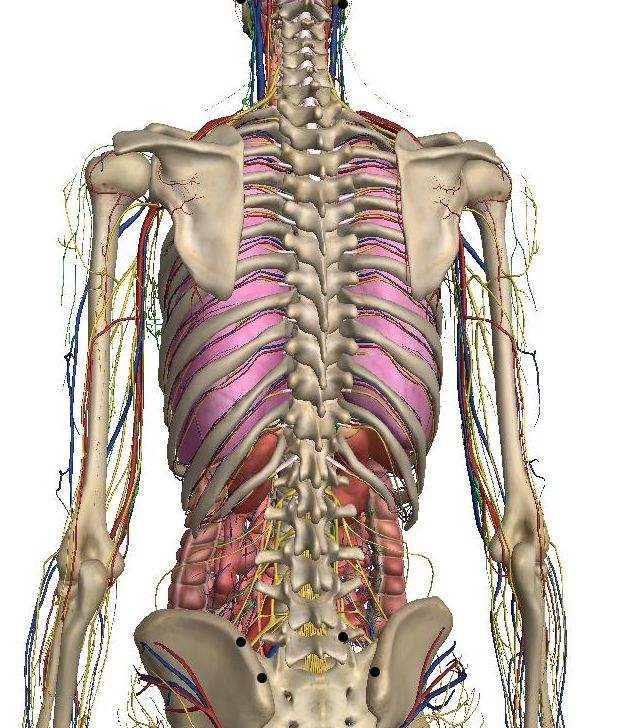
\includegraphics[height=0.4\linewidth]{figures/2-bg/zygote-body-back}}
\caption{Anatomy 3D models from Zygote\protect\footnotemark.}
\label{fig:2-bg:zygote-body-esplorazione}
\end{figure}
\footnotetext{\url{www.zygotebody.com}}
Many of them offer interactive anatomy models, usable either as an on-line service or as a standalone application. There also exist organizations specifically offering teaching bundles for use in classrooms, making it possible to use alternative teaching methods at different school levels assisted by videos and interactive tools. Those interactive applications offer large improvements over the classical method. It is possible to view organs and structures from any desired angle, control magnification and often even select specific organs and systems to be displayed or hidden. 
Many commercially available systems use VR for medical education and psychomotor skills training \cite{Lu2005,Basdogan2007}. These systems have indeed proven to be valid and useful.
By combining computer models of anatomical structures with custom software we can showcase to students new ways of interacting with anatomy that could not be achieved during cadaveric dissections or in static diagrams and models for increasing their learning satisfaction \cite{Bacca2014}. 
Visualization of medical data can also be used for education. Medical datasets are very large and the visualization must correctly represent the reality. Today images with a very high level quality can be generated by high performance graphics for computer gaming (see \figurename{\ref{fig:2-bg:CTRendering}}).  
\begin{figure}
\centering  %http://the-science-llama.tumblr.com/post/44636847547/staceythinx-volume-rendering-ct-scans-by
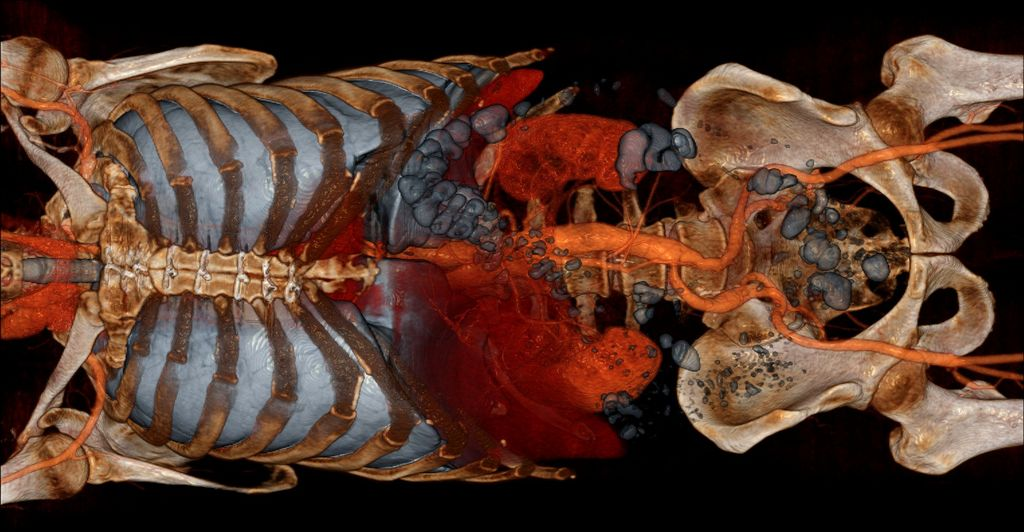
\includegraphics[width=0.8\linewidth]{figures/2-bg/CTRendering}
\caption{Recent CT volume visualization.}
\label{fig:2-bg:CTRendering}
\end{figure}

Through all those materials and interactive elements, the users can control the region of interest and hopefully better understand the information they are looking for. 
These resources are very valuable and are more interactive and interesting than textbooks, however, with the disadvantage of having users still mentally map/link anatomy onto their bodies.
Humans usually have to build the knowledge network in the brain after perception of the knowledge. The information is very general but the learning procedure is quite personal. Personalized information is much easier for the user to accept.
Fresh medical students still bear a very long and hard study during the medical knowledge transferring.
At the same time, different technology is developed to simplify the learning tasks.
% However, digital methods find increasing popularity among medical teaching institutions.
%Overall, anatomy within medical education has seen a significant decline in content delivered and learning time \cite{Patel2008}. 

\subsection{Public and patient education}
For obvious reasons, methodologies for medical education are not suitable for public education, as it is not necessary to teach a high-level of anatomy understanding. 
However, real-life demonstrations are limited to the skin-surface, which is why most people learn about anatomy in the form of charts or plastic models of the inner organs. Still, there is a certain fascination about looking into the inside of one's own body, something that can usually only be achieved to a limited degree by the use of X-Ray imaging or similar imaging modalities. Those methods are usually not applicable for educational methods, mostly because the devices are too expensive to use without medical indication and for certain methods there are risks like irradiation or injection of tracer materials.

Patient education is the process by which health professionals and others impart information to patients and their caregivers that will alter their health behaviors or improve their health status.%\footnote{\url{https://en.wikipedia.org/wiki/Patient_education}}. 
It can improve the patient's understanding of medical condition, diagnosis, disease, or disability. Patient education is an important and often underestimated responsibility of a health professional \cite{Waitzkin1984}.
It is the responsibility of a doctor to inform and motivate patients to ensure that they understand the diseases, the treatment options available and the consequences of no treatment or non-compliance \cite{Fenol2010}. This makes it possible for the patients to understand it, eventually allowing them to take responsibility for their own health \cite{Ammann2010}. Good information and communication increases the patient's possibility to contribute in the decision-making process, leading to higher levels of patient satisfaction, loyalty to the physician and favouring treatment outcomes \cite{Huber2012b,Ammann2010,Cleeren2014}. 
\begin{figure}
	\centering
	\subfloat[Using Atlas.]{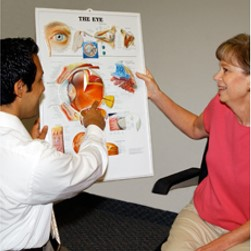
\includegraphics[height=0.4\linewidth]{figures/2-bg/patientEducation1}
		\label{fig:2-bg:patientEducation:atlas}}
	\quad
	\subfloat[Multimedia.]{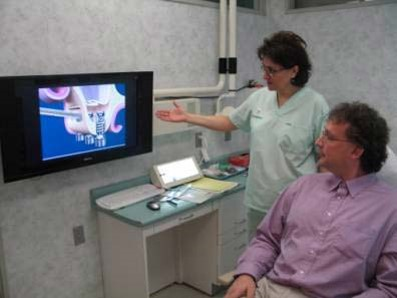
\includegraphics[height=0.4\linewidth]{figures/2-bg/patientEducation2}
		\label{fig:2-bg:patientEducation:video}}
	\caption{Patient education scenarios.}
	\label{fig:2-bg:patientEducation}
\end{figure}
Traditionally, patient-health professional communication in a clinical setting comprises of a face-to-face narrative interaction often combined with static images or real-time sketching (see \figurename{\ref{fig:2-bg:patientEducation:atlas}}). 
%While it is important to have a patient fully informed and engaged in the decision-making process, 
It is inevitable that patients' comprehension of explanations is often lacking due to the complexity of the medical information \cite{Cleeren2014}. Evidence suggests that patients often do not understand what is being said to them when information is given during a medical encounter due to cultural and educational gaps between clinicians and patients \cite{Beranova2007}. This discourages the patient and leaves them overly reliant on their doctor's advice.

Improving and facilitating the information process and understanding by the patient has been a focus of research in the medical field. 
\citet{Ong1995} presented a literature survey of doctor-patient communication, summarizing the key topics of information exchange, interpersonal relationship building, and shared medical decision making. \citet{Wilcox2010a} proposed a design for patient-centric information displays to deliver useful information to a patient during an emergency room visit, since the patients are frequently underinformed. Previous work has also demonstrated that technology can positively impact communication. \citet{Hsu2005} conducted a longitudinal study the impact of in-room access to electronic health records on doctor-patient interactions during outpaitent visits.
%For example, the European Federation of Periodontology made video information for patients available on their website. 
%Despite the availability of different 3D multimedia patient education computer programs, the use of these programs is not generalized. 
Recent reviews show growing evidence with regards to the benefit of multimedia tools in enhancement of patients' satisfaction and improvement of knowledge retention \cite{Beranova2007}. 
\add{A patient education computer program using 3D multimedia videos is shown in \figurename{\ref{fig:2-bg:patientEducation:video}}.}
In addition, 3D animations have been suggested, for educating audiences that are preliterate or have limited literacy skills, such as children with mental handicaps \cite{T.1997} and to be useful for patients with a lower learning pace as it leads to a better understanding of the disease \cite{Jimison1998}. 
%Currently, most clinical settings are still without the use of this new technology to assist in the process of informing patients about the diseases and different procedures. 
\citet{Ni2011} presented the design, development, and evaluation of AnatOnMe, a projection-based handheld device designed to facilitate medical information exchange (see \figurename{\ref{fig:2-bg:AnatOnMe-projection-basedhandhelddevice}}). Adopting a user-centered design approach, they interviewed medical professionals to understand their practices, attitudes, and difficulties in exchanging information with patients, as well as to identify their workflow, tasks, and design requirements for a technology intervention.
\begin{figure}
\centering
\includegraphics[width=0.85\linewidth]{"figures/2-bg/AnatOnMe-projection-based handheld device"}
\caption{AnatOnMe in use in a simulated physical therapy consultation. The physical therapist explains a knee injury to his patient using on-body projection of medical imagery.}
\label{fig:2-bg:AnatOnMe-projection-basedhandhelddevice}
\end{figure}

\citet{Gonzales2012} presented an application that personalized the content presented on the device to the patient's diagnosis in an easy-to-understand language, rather than hard-to-understand medical terminology, and encourages patient-physician interaction on the main topical areas of a patient's diagnosis.
\citet{Ihrig2012} evaluated the view of physicians performing multimedia supported preoperative education within a randomized controlled trial, enrolling 8 physicians and 203 patients, and patients and physicians profited from multimedia support for education and counseling without prolonging patient education. 


\subsection{Rehabilitation exercise}
Rehabilitation is the process to regain full function following injury\footnote{\url{http://www.sportsinjuryclinic.net/rehabilitation-exercises}}. This involves restoring strength, flexibility, endurance and power and is achieved through various exercises and drills (see \figurename{\ref{fig:2-bg:rehabilitation}}). Rehabilitation is as important as treatment following an injury but unfortunately is often overlooked. Usually physiatrists are involved in the exercise procedure and optimal physical activities are carried out in an effort to reach specific health goods. Its purpose is to return to normal musculoskeletal function or to decrease pain caused by injuries or other health problem. 

The communication between a medical assistant and a patient is very important during the exercise, \eg make sure that the patient knows the current state of his/her disability and follows guidelines during the rehabilitation exercise. The rehabilitation process is commonly performed in a rehabilitation center, and the physiotherapist identifies and evaluates the movements and motor functions that are being affected. In order to achieve kinetic gains as quickly as possible, patients are encouraged to perform the same exercise movements several times \cite{Metcalf2013}. Patients' learning by movement repetition is crucial for their successful therapy. The time that the patient expends in the rehabilitation center is relatively short compared with the time he/she spends at home with no supervision \cite{Crocher2013}. However, there are some issues with home exercises:(i) the patient cannot be motivated by the therapist, and (ii) wrong movements might be performed without timely correction.

\begin{figure}
	\centering
	\subfloat{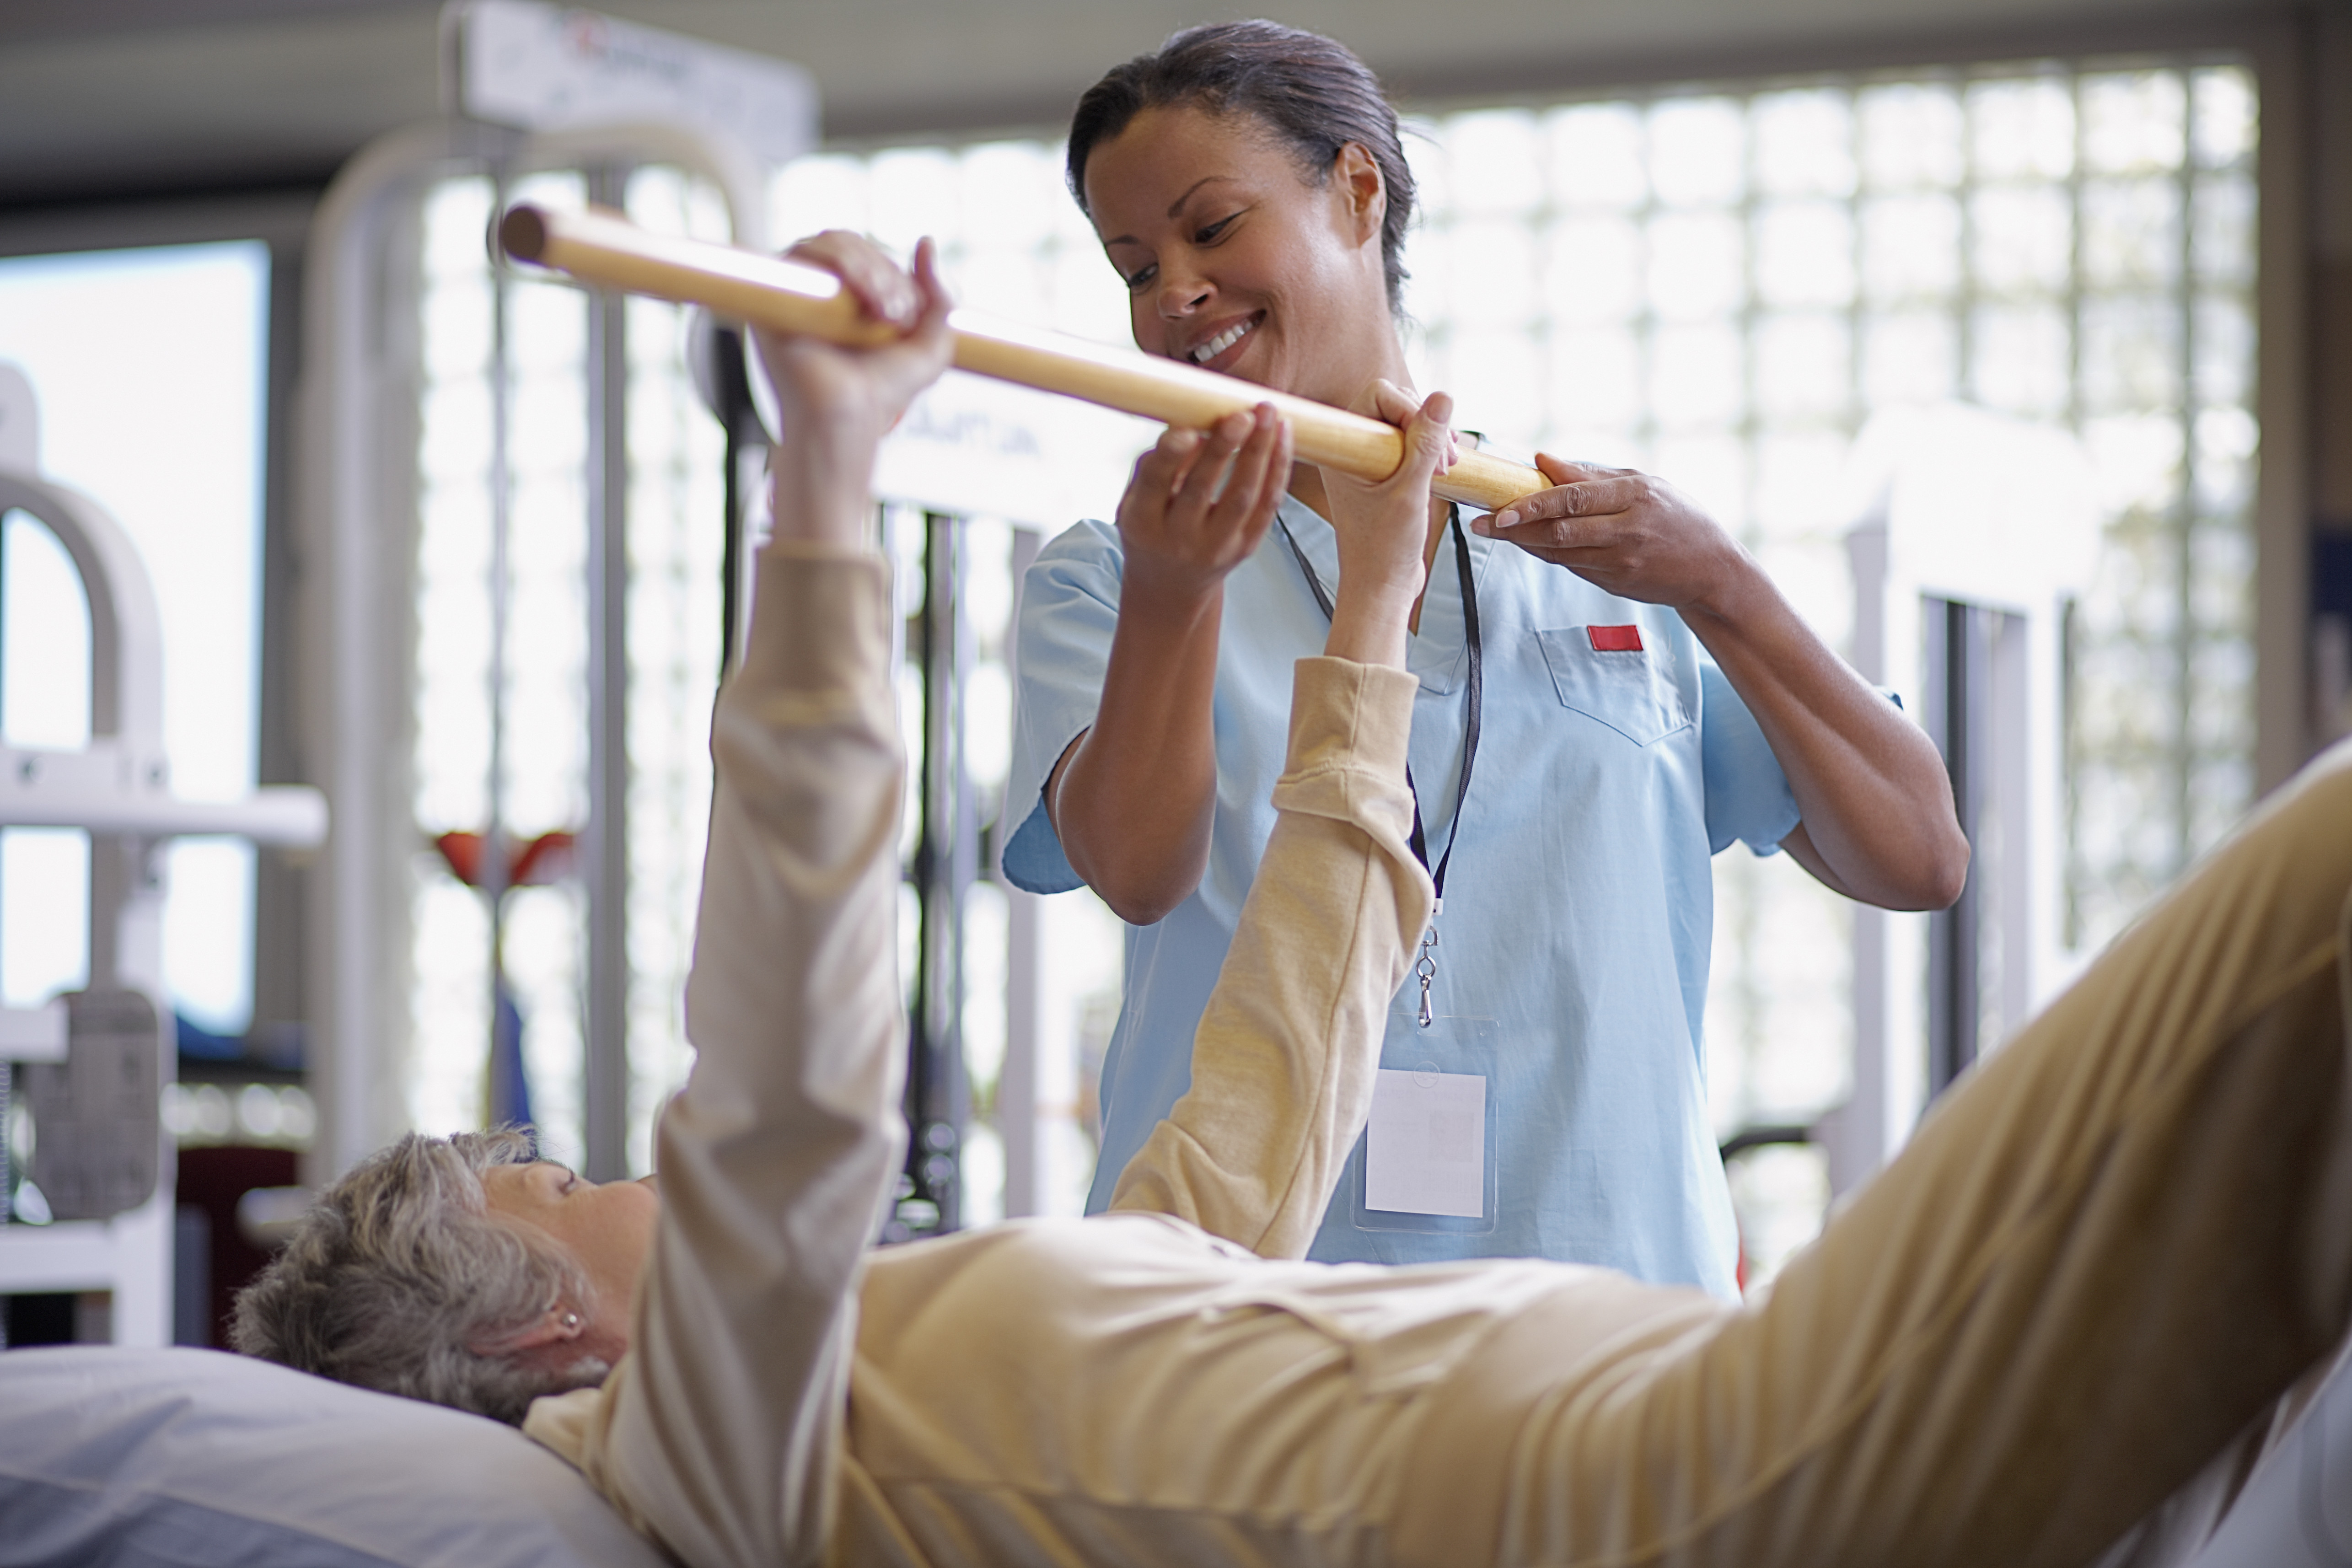
\includegraphics[height=0.3\linewidth]{figures/2-bg/rehabilitation}}
	\qquad
	\subfloat{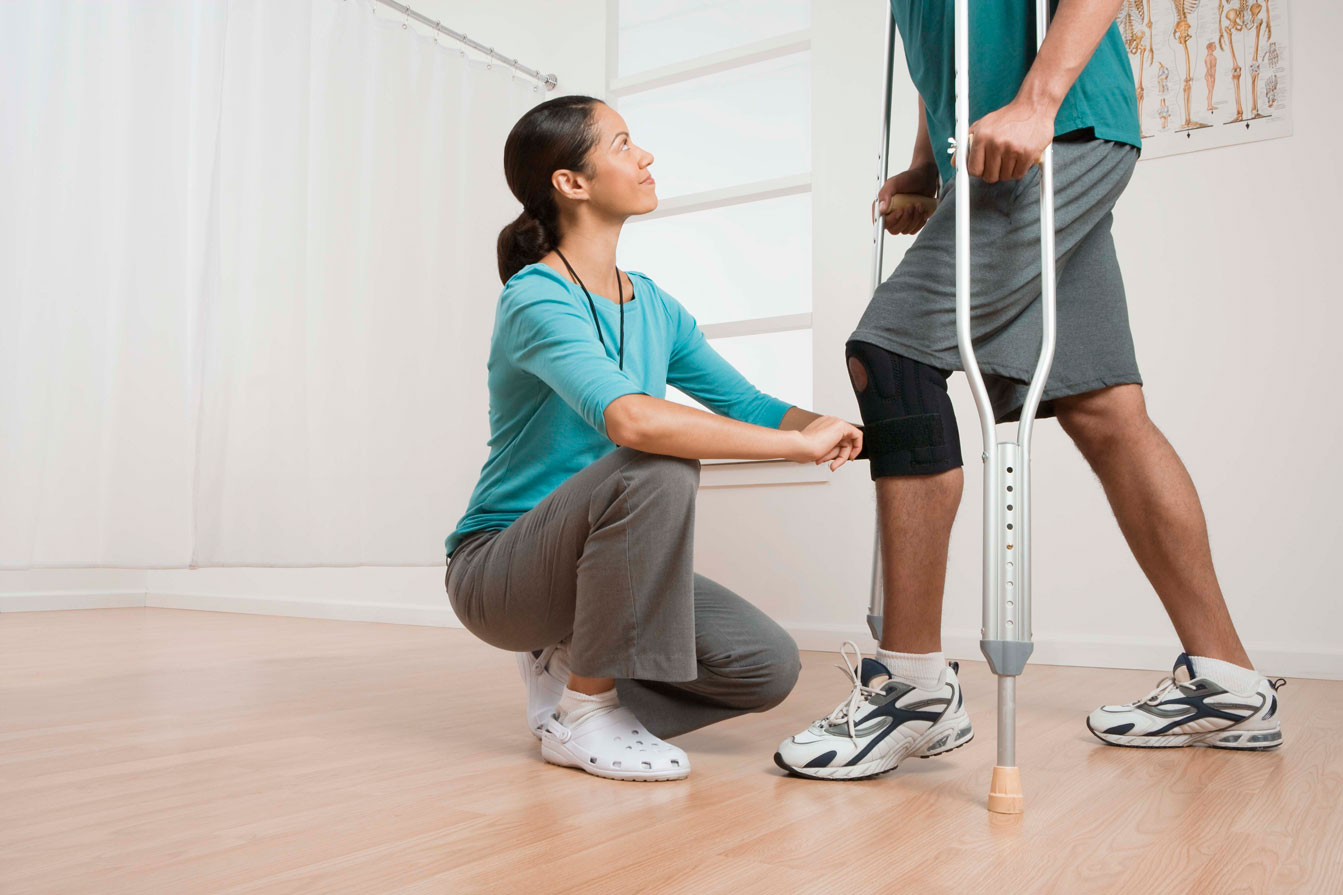
\includegraphics[height=0.3\linewidth]{figures/2-bg/rehabilitation2}}
	\caption{Rehabilitation Exercise. Usually physiatrists are involved in the exercise procedure and optimal physical activities are carried out in an effort to reach specific health goods.}
	\label{fig:2-bg:rehabilitation}
\end{figure}

Today, interactive solutions for rehabilitation are being developed using different sensors and motion tracking systems including gloves, magnetic, fiducial or infrared markers, video and depth cameras, and VR and AR systems are introduced to motivate the patient and facilitate a more accurate exercise \cite{DaGama2015,Cho2014}. 
The activity of patients' muscles can be visualized and the movement is checked based on the contracted muscles \cite{Woodford2007}. \citet{Cho2014} developed a virtual reality proprioception rehabilitation system for stroke patients to use proprioception feedback in upper limb rehabilitation by blocking visual feedback.
The markerless tracking feature of Kinect enables a natural user interaction for rehabilitation applications, which alleviates existing issues for patients having difficulty to hold any sensor or marker. Using Kinect, various research are being explored for the development of assistive systems that help interact with patients during their rehabilitation exercises \cite{Cordella2012, Gama2012a, Anton2013, Borghese2013}.

\subsection{Intra-operative interaction with medical information}
%\subsection{special requirements for interaction}
As medical technology is continuously developing, more medical systems are used not only in diagnosis but also during surgery. In a modern Operating Room (OR), the surgeon completes the operation with the help of different medical systems and quite a few interactions have to be performed by the surgical team to control the corresponding medical systems and retrieve the desired information (see \figurename{\ref{fig:1-intro:ORScenario}}).
The key to successful minimally-invasive procedures is immediate access to the patient's medical imaging data during the intervention. In contrast to open surgery, physicians are not able to see their target, surrounding risk structures or their instruments inside the patient and therefore rely heavily on intra-operatively acquired medical images. Because of special working conditions in the OR, i.e. sterility, limited space and time pressure, physicians face challenging human-computer interaction tasks. These tasks include the control of medical image viewers, interactive registration of images, and interaction with medical robots. In clinical routine, sterile covers enable the direct use of interaction devices, e.g. joystick, touchscreen or control panel. In addition, foot pedals are used to control software directly. In contrast, the interaction with software is very often delegated to a non-sterile assistant using speech or gesture commands \cite{Hubler2014}.
It is a big challenge for the surgical team to manage and naturally interact with all the medical information in OR.

Giving the surgeon direct control of the interaction of different medical systems while maintaining sterility within the operating room, has captured the imagination of many research groups, and different solutions have been proposed. 
One approach is to insert a barrier between the sterile gloves and the non-sterile input device \cite{Ionescu2006}. This solution is very simple but involves certain inherent risks due to the potential damage to the barrier. Computer vision techniques are also being used to introduce interaction methods in the operating room that avoid the need for contact with an input device.
A non-contact mouse was developed in \cite{Gratzel2004a} using a stereo camera that provided the surgeon standard mouse functions to control a single medical system. Even if they only developed simple gestures to control the cursor movement and clicking, the interactions were not performed smoothly. It also required each medical system to be augmented by a pair of stereo cameras which increases the hardware complexity in the OR (see \figurename{\ref{fig:2-bg:touchlessMouse}}). 
\begin{figure}
	\centering
	\subfloat{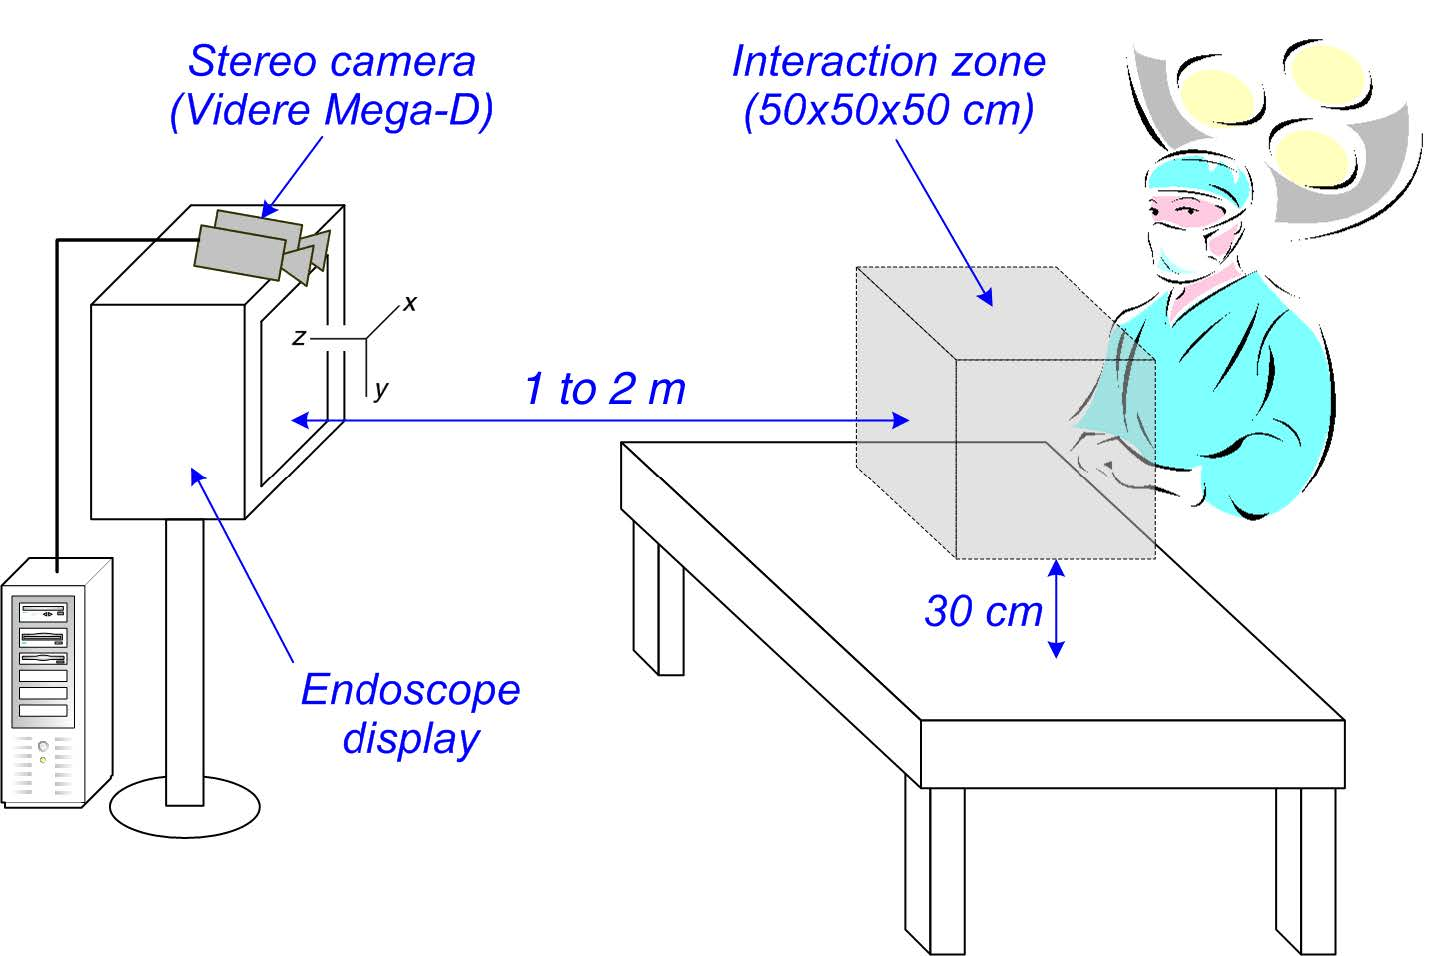
\includegraphics[height=0.3\linewidth]{figures/2-bg/touchlessMouse1}}
	\qquad
	\subfloat{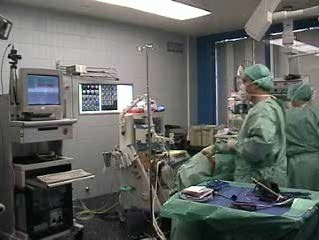
\includegraphics[height=0.3\linewidth]{figures/2-bg/touchlessMouse2}}
	\caption{Touchless Mouse. A non-contact mouse was developed using a stereo camera, providing the surgeon standard mouse functions to control a single medical system.}
	\label{fig:2-bg:touchlessMouse}
\end{figure}
Washs \textit{et al.} \cite{Wachs2008} developed more sophisticated gestures for image browsing.
Quite a few touchless systems \cite{Strickland2013,Ebert2013,Tan2013} for the OR were developed after the Kinect sensor was released, as it has lower barriers and could be easily adapted.
Ebert \textit{et al.} \cite{Ebert2013} presented a system which allowed the control of the open source Picture Archiving and Communication System (PACS) OsiriX by means of gesture and voice commands.   
The system in \cite{Strickland2013} helped navigate a predefined stack of MRI/CT images, using a simple constrained gesture set to move forward or backward through the image slices. 
The work in \cite{Tan2013} built compound gestures that combined dominant and non-dominant hand, which were used for selecting, and other particular functions and modes. 
Once Leap Motion {(California, United States)} commercially appeared, a custom workstation was also set up in order to manipulate the imaging software by hand gestures \cite{Rosa2014}. 
All these systems have a similar setup, since a depth sensor is placed next to the screen to perform outside-in tracking while observing the surgeon to detect the gestures which are subsequently mapped to different functions. 

\citet{Jalaliniya2013} presented user interfaces for gesture-based interaction with medical images via a wristband sensor or capacitive floor sensors (see \figurename{\ref{fig:2-bg:HandFootGesture}}). However, interaction with medical images or systems in a surgical setting often extends beyond simple navigation, requiring a much richer set of image manipulation options. 
Along with the larger gesture sets enabled by this expressiveness comes concern over the learnability of the system - natural user interfaces are not natural any more \cite{Norman2010a,Schwarz2011a}. 
Several strategies have been also explored for touchless interaction with medical images, through speech recognition and egocentric interaction. 
Speech recognition is used in \cite{Ebert2012}, however voice-recognition software involves special challenges in noisy operating rooms and often are exhausting when repeated frequently during surgeries throughout the day. The egocentric interaction paradigm \cite{Pederson2010} redefines the relationship between the human, computer system, and world, hence a wearable personal prototype for surgeons was developed based on Google Glass \cite{Jalaliniya2015}.
A set of socio-technical issues, or human factors, arose when the above systems were used in the context of an actual surgery, including collaboration, engagement and disengagement.
\begin{figure}
	\centering
	\subfloat[System Architecture.]{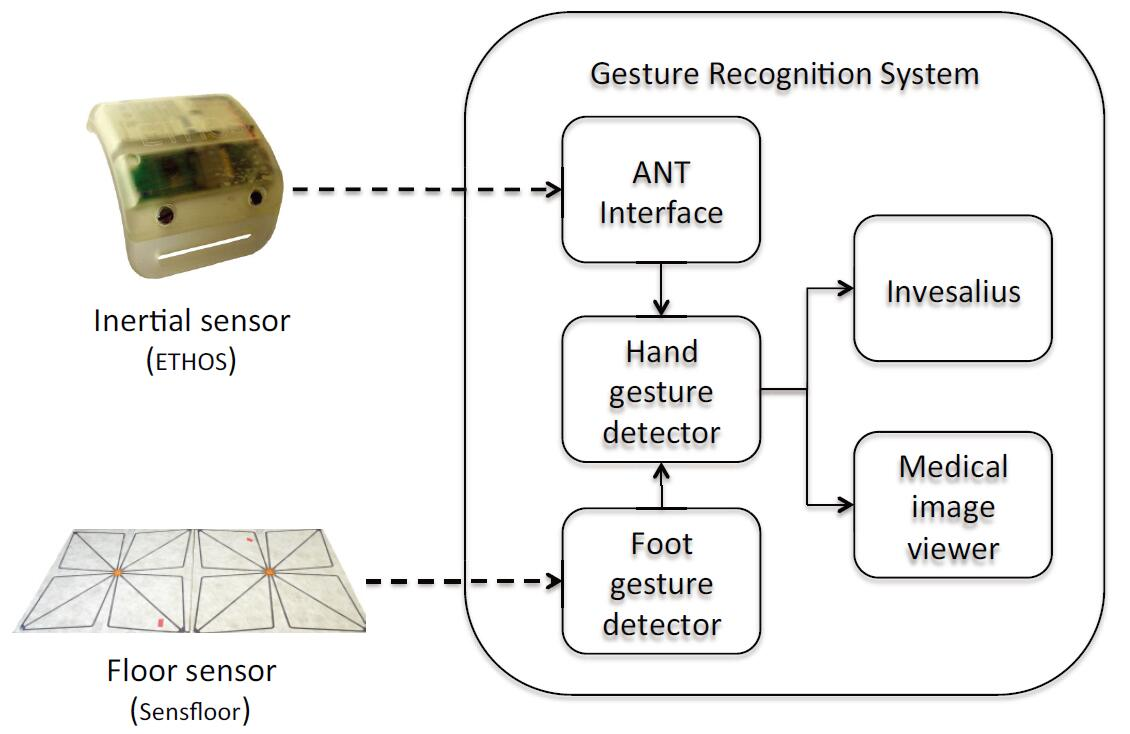
\includegraphics[height=0.3\linewidth]{figures/2-bg/HandFootGesture0}}
	\qquad
	\subfloat[A user interacting with the system.]{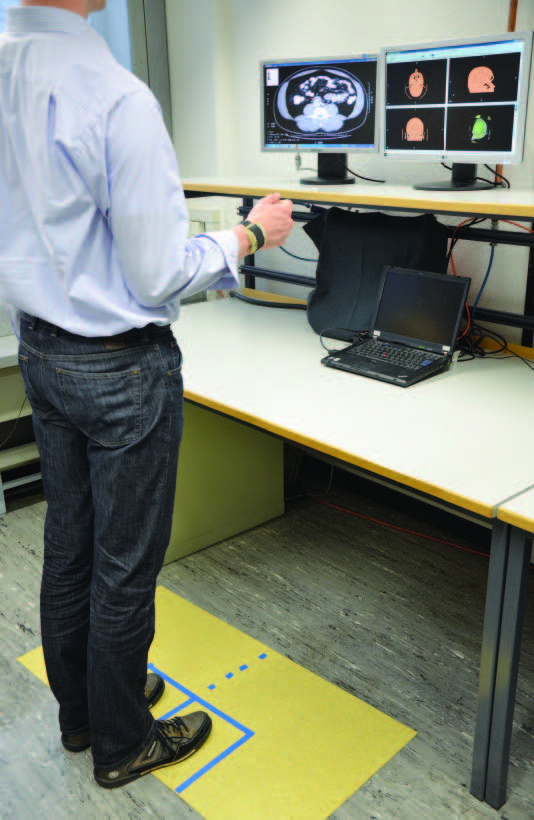
\includegraphics[height=0.3\linewidth]{figures/2-bg/HandFootGesture}}
	\caption{Touch-less interaction with medical images using hand\&foot gestures.}
	\label{fig:2-bg:HandFootGesture}
\end{figure}

\section{Mixed Reality Environment}
Mixed reality is the merging of real and virtual worlds to generate new environments and visualizations where physical and digital objects co-exist and interact in real time%\footnote{\url{https://en.wikipedia.org/wiki/Mixed_reality}} 
and it encompasses both augmented reality and augmented virtuality (AV), as shown in \figurename{\ref{fig:2-bg:Reality-Virtuality_Continuum}}. MR environment is defined as one in which real world and virtual world objects are presented together, that is, anywhere between the extrema of the RV continuum \cite{Milgram1994a}. 
\begin{figure}
	\centering
	
\includegraphics[width=0.8\linewidth]{figures/2-bg/Reality-Virtuality_Continuum}
	\caption{Reality-Virtuality (RV) Continuum}
	\label{fig:2-bg:Reality-Virtuality_Continuum}
\end{figure}
Usually the MR environment is created via a MR/AR application, which combines the real world and virtual world through an AR view.
MR/AR applications provide a basis for embedding content perceptually within the environment, either by direct augmentation or via a 3D model of it. Both these application types use the world as the user interface, thereby potentially minimizing the need for spatial inferencing and cue-based triangulation for simple short-distance target finding tasks. The advantages of MR environment are to improve the perception of the ambient information with the corresponding interactive methods \cite{Nurminen}. In this section, we first examine the states of augmented reality and Medical AR application, then simply discuss collaborative mixed reality and serious gaming.

\subsection{Augmented Reality}
Augmented Reality supplements the real scene with virtual elements, creating a MR environment. It has been widely used in areas such as training and education, manufacturing and repair, annotation and visualization, robot path planning, entertainment, and military aircraft guidance \cite{Krevelen2010}.
In AR, artificial, computer generated content is used to enrich or annotate the real world. AR techniques are inherently egocentric. Augmentations lie either directly in the view of the user (using see-through displays) or on top of a camera view \cite{Karimi2004}. 
An AR system has three key characteristics: (a) it mixes real and virtual imagery, (b) registers the digital data to the real world, and (c) provides interactivity in real-time \cite{Azuma1997a}. AR in formal and informal MR environments with an emphasis on affordances, usually utilizes context-aware technologies, which enable participants to interact with digital information embedded within the physical environment \cite{Dunleavy2008}. The AR system presents digital media to users after they point the camera at an object (e.g., QR code, 2D target) and creates immersible learning experiences with the physical environment, providing a novel and potentially transformative tool for learning, training, navigation and so on \cite{Dede2009,Johnson2011}.

One of the main challenges is accurate registration, where the virtual content is accurately positioned onto the real world. Two fundamental methods for this are commonly utilized: 1) sensor-based registration and 2) computer vision based registration. 
Typical computer vision based AR systems use fiducial markers for tracking. Recently, research has focused in markerless environments. These approaches have their pros and cons. Sensor-based registration is globally applicable, but depends on sensor accuracy. For markerless recognition, visual features from areas and targets to be recognized need to be pre-extracted. 
Another challenge is the correct perception of augmentations, related to environments, capturing, augmentation, display, and individual user differences  \cite{Kruijff2010}.
 

\subsubsection{Tracking via RGB-D sensors}
A RGB-D sensor provides synchronized color and depth images and is frequently employed as an input and tracking device in the AR system. 
There are RGB-D sensors with different techniques, such as stereo cameras, time-of-flight (TOF) cameras, and structured light. There are several popular sensors available, with different size and power consumption, and the popular devices are Intel RealSense 3D Camera, Asus Xtion LIVE PRO for laptops, and Microsoft Kinect versions 1 and 2 for desktop.
Each sensor's specification is shown in \tablename{ \ref{tb:2-bg:RGBDSensors}}. 
\begin{table}
	\caption{Specification of RGB-D Sensors. RealSense is very light, while Kinect v2 is heavier and has much higher power consumption.}
	\label{tb:2-bg:RGBDSensors}
	\scriptsize
	\centering
	\begin{tabular}{P{2cm}|P{2cm}|P{2cm}|P{2cm}|P{2cm}}
		\hline
		\space & RealSense & Xtion & Kinect V1 & Kinect V2 \\
		\hline
		Weight (pound) & 0.077 & 0.5 & 4 & 4.5\\
		\hline
		Size (inch) &5.2x0.25x0.75 & 7.1x1.4x2 & 11x2.3x2.7 & 9.8x2.7x2.7 \\
		\hline
		power & 2.5W USB & 2.5W USB & 12.96W & 115W \\
		\hline
		technology & TOF & structured light & structured light & TOF \\
		\hline
		depth resolution & 628x468 & 640x480 & 640 x480 & 512z424 \\
		\hline
		color resolution & 1920x1080 & 640x480 & 640x480 & 1920x1080 \\
		\hline
		tracked objects & face and hand & human body & human body & human body \\
		\hline
	\end{tabular}
\end{table}

The Kinect V1 sensor introduced by Microsoft in 2010 is evidently a breakthrough that brings low-cost 3D depth sensing and human body pose estimation technologies to the public \cite{Zhang2012b}. 
Since Kinect's launch date, it has been exploited in all kinds of computer gaming and mixed reality applications. 
Hence, we only examine the Kinect V1 for technologies of the depth sensor and human skeletal tracking.
The Kinect V1 sensor incorporates several advanced sensing hardware. Most notably, it contains a depth sensor, a color camera, and a four-microphone array that provide full-body 3D motion capture, facial recognition, and voice recognition capabilities (see \figurename{\ref{fig:2-bg:kinect}}). Here we only focus on the main technologies, depth sensor and human skeletal tracking, and some technologies to collect more personal information.
\begin{figure}
	\centering
	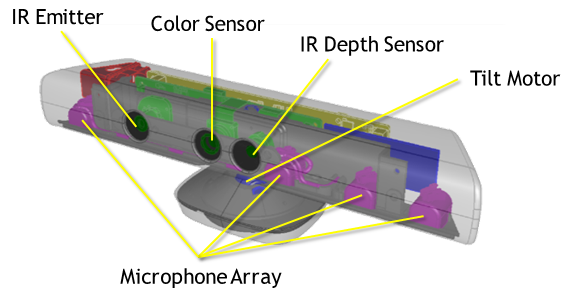
\includegraphics[width=0.7\linewidth]{figures/2-bg/kinect}
	\caption{Kinect for Windows Sensor Components. There is an RGB camera, an infrared emitter and IR depth camera, a multi-array microphone, and a 3-axis accelerometer.}
	\label{fig:2-bg:kinect}
\end{figure}

\paragraph{Depth sensor}
\figurename{\ref{fig:2-bg:kinect}} shows the arrangement of the infrared (IR) projector, the color camera, and the IR camera. The depth sensor consists of the IR projector combined with the IR camera, which is a monochrome complementary metal-oxide semiconductor (CMOS) sensor. The depth-sensing technology is licensed from the Israeli company PrimeSense\footnote{\url{www.primesense.com}}. Although the exact technology is not disclosed, it is based on the structured light principle. The IR projector is an IR laser that passes through a diffraction grating and turns into a set of IR dots. The relative geometry between the IR projector and the IR camera as well as the projected IR dot pattern are known. If we can match a dot observed in an image with a dot in the projector pattern, we can reconstruct it in 3D using triangulation. Because the dot pattern is relatively random, the matching between the IR image and the projector pattern can be done in a straight forward way by comparing small neighborhoods. The depth values from Kinect do not have the same accuracy. Depth is determined through triangulation, similar to stereovision. The depth error increases with the distance squared.
A point cloud can be generated from the depth image to implement tracking and 3D reconstruction. The influential KinectFusion system \cite{Newcombe2011} demonstrated real-time depth camera tracking and dense scene reconstruction by registering incoming depth images to a volumetric representation of the scene. \citet{Schulman2013} introduced an algorithm for tracking deformable objects from a sequence of point clouds, which is based on a probabilistic generative model that incorporates observations of the point cloud and the physical properties of the tracked object and its environment.
\citet{Zhou2015} presented an approach for tracking camera pose in real time given a stream of depth images via useful contour cues.

\paragraph{Human skeletal tracking}
The innovation behind Kinect hinges on advances in human skeletal tracking. 
The demands for commercially viable skeletal tracking are enormous. 
Simply put, skeletal tracking must ideally work for every person on the planet, in every house-hold. A dauntingly high number of dimensions describe this envelope, such as the distance from the Kinect sensor and the sensor tilt angle. 
Entire sets of dimensions are necessary to describe unique individuals, including size, shape, hair, clothing, motions, and poses. Household environment dimensions are also necessary for lighting, furniture and other household furnishings, and pets.
However, in this skeletal tracking technology a human body is represented by a number of joints representing body parts such as head, neck, shoulders, and arms(see \figurename{\ref{fig:2-bg:skeleton:a}}). Each joint is represented by its 3D coordinates. The goal is to determine all the 3D parameters of these joints in real time to allow fluent interactivity and with limited computational resources. 
Rather than trying to determine directly the body pose in this high-dimensional space, the Kinect team met the challenge by proposing per-pixel, body-part recognition as an intermediate step (see \figurename{\ref{fig:2-bg:skeleton:b}}) \cite{Shotton2011}. With the 3D human skeletal tracking algorithm, it enables quite a few personalized AR applications and interaction between users and visual and physical objects without the need of touching and markers.
\begin{figure}
	\centering
	\subfloat[Using a skeletal representation of various body parts.]{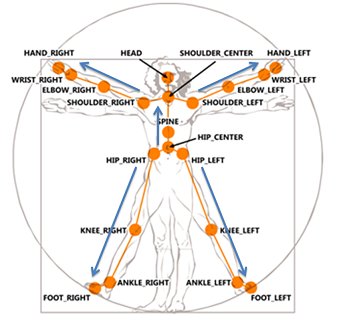
\includegraphics[height=0.35\linewidth]{figures/2-bg/kinectSkeleton} \label{fig:2-bg:skeleton:a}}
	\quad
	\subfloat[Kinect uses per-pixel, body-part recognition as an intermediate step to avoid a combinatorial search over the different body joints.] {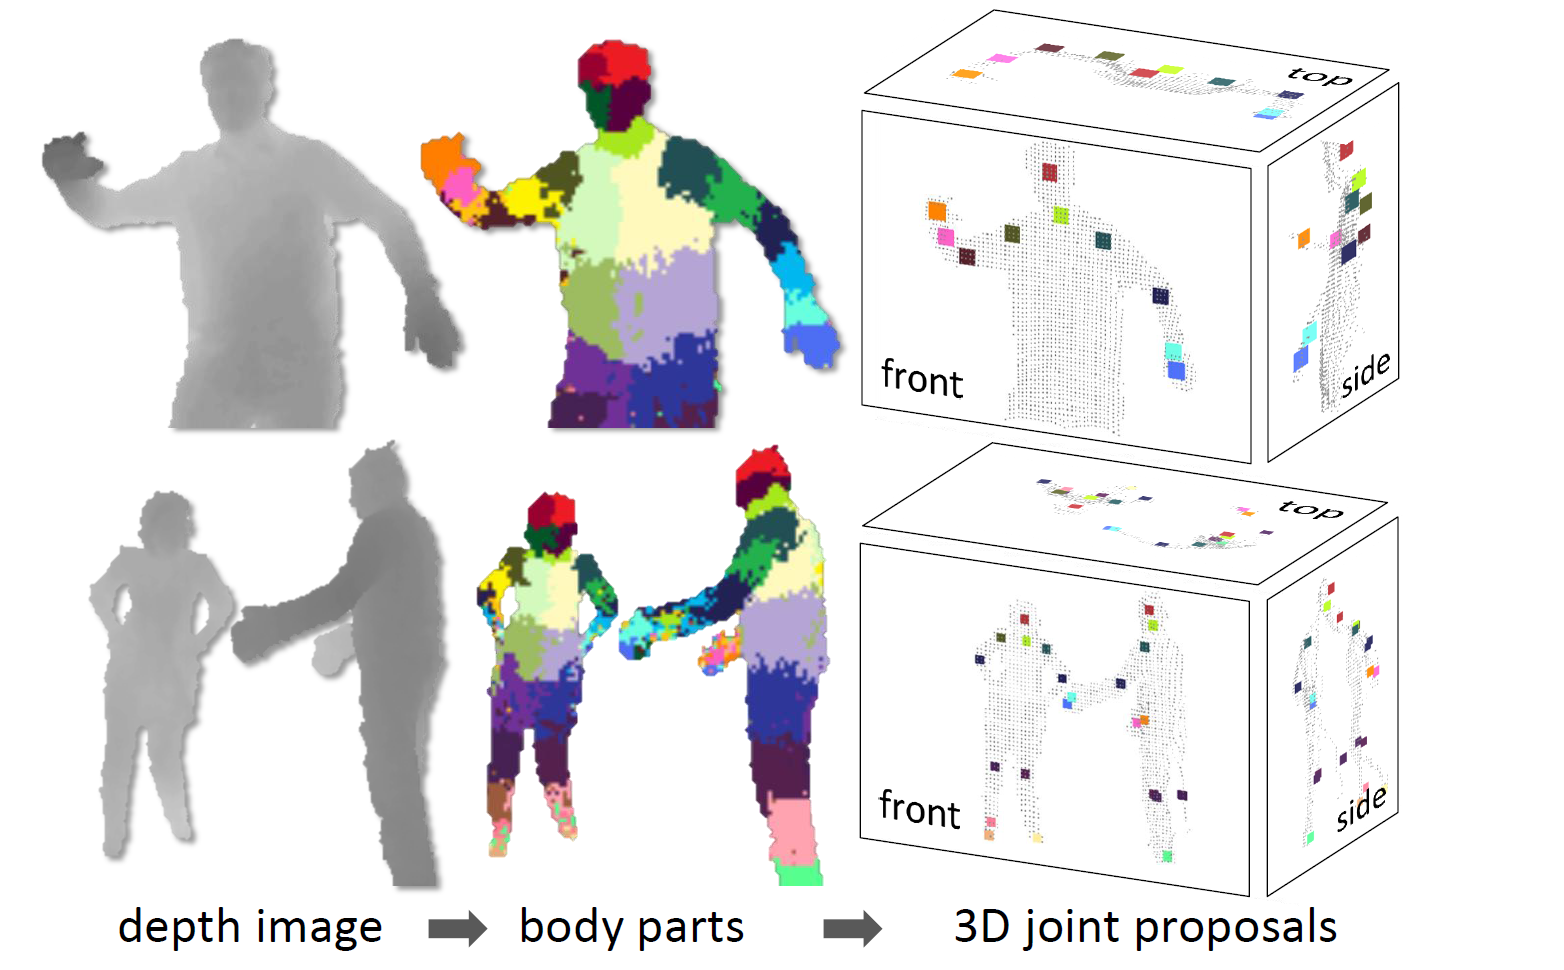
\includegraphics[height=0.35\linewidth]{figures/2-bg/kinectDepthSkeleton} \label{fig:2-bg:skeleton:b}}
	\caption{Skeletal tracking. From a single input depth image, a per-pixel body part distribution is inferred. (Colors indicate the most likely part labels at each pixel, and correspond in the joint proposals). Local modes of this signal are estimated to give high-quality proposals for the 3D locations of body joints, even for multiple users.}
	\label{fig:2-bg:skeleton}
\end{figure}

\paragraph{Personal information} %from the True AR paper
As technologies improve, the perception and interaction with the digital information is more and more natural. These include the user's personal behaviors, thus personal information should be collected to improve the user's experience in the MR environment.
The user is the final stage of the perceptual pipeline and the perception of the digital content presented in the MR environments can be highly influenced by individual differences between users. 
These differences may require noticeable modifications in the way the virtual information in presented \cite{Kruijff2010}.
Personal information usually includes gender, age, weight, size, and body shape. 
Based on the skeletal tracking, computing has to be done to detect more information from the image device. 
The Open Source Biometric Recognition (OpenBR)\footnote{\url{http://openbiometrics.org}} is a communal biometrics framework supporting the development of open algorithms and reproducible evaluations \cite{Klontz2013}. 
%The basic algorithm used in the OpenBR is the Spectrally Sampled Structural Subspaces Features (4SF) algorithm. 
The algorithm is based on the statistical learning methods and used in the field of demographics and aging using face recognition concepts. (see \figurename{\ref{fig:2:OpenBR}}). It is easy to use and fairly precise with 92.8\% accuracy of the gender estimation, 9.9 years RMS error of males and 12.8 years RMS error of female. In addition, ReconstructMe\footnote{\url{http://reconstructme.net/reconstructme-sdk/}} is a powerful and affordable real-time 3D reconstruction system. Quite a few personal information can be detected from the 3D reconstruction of the human body.
\begin{figure}
	\centering
	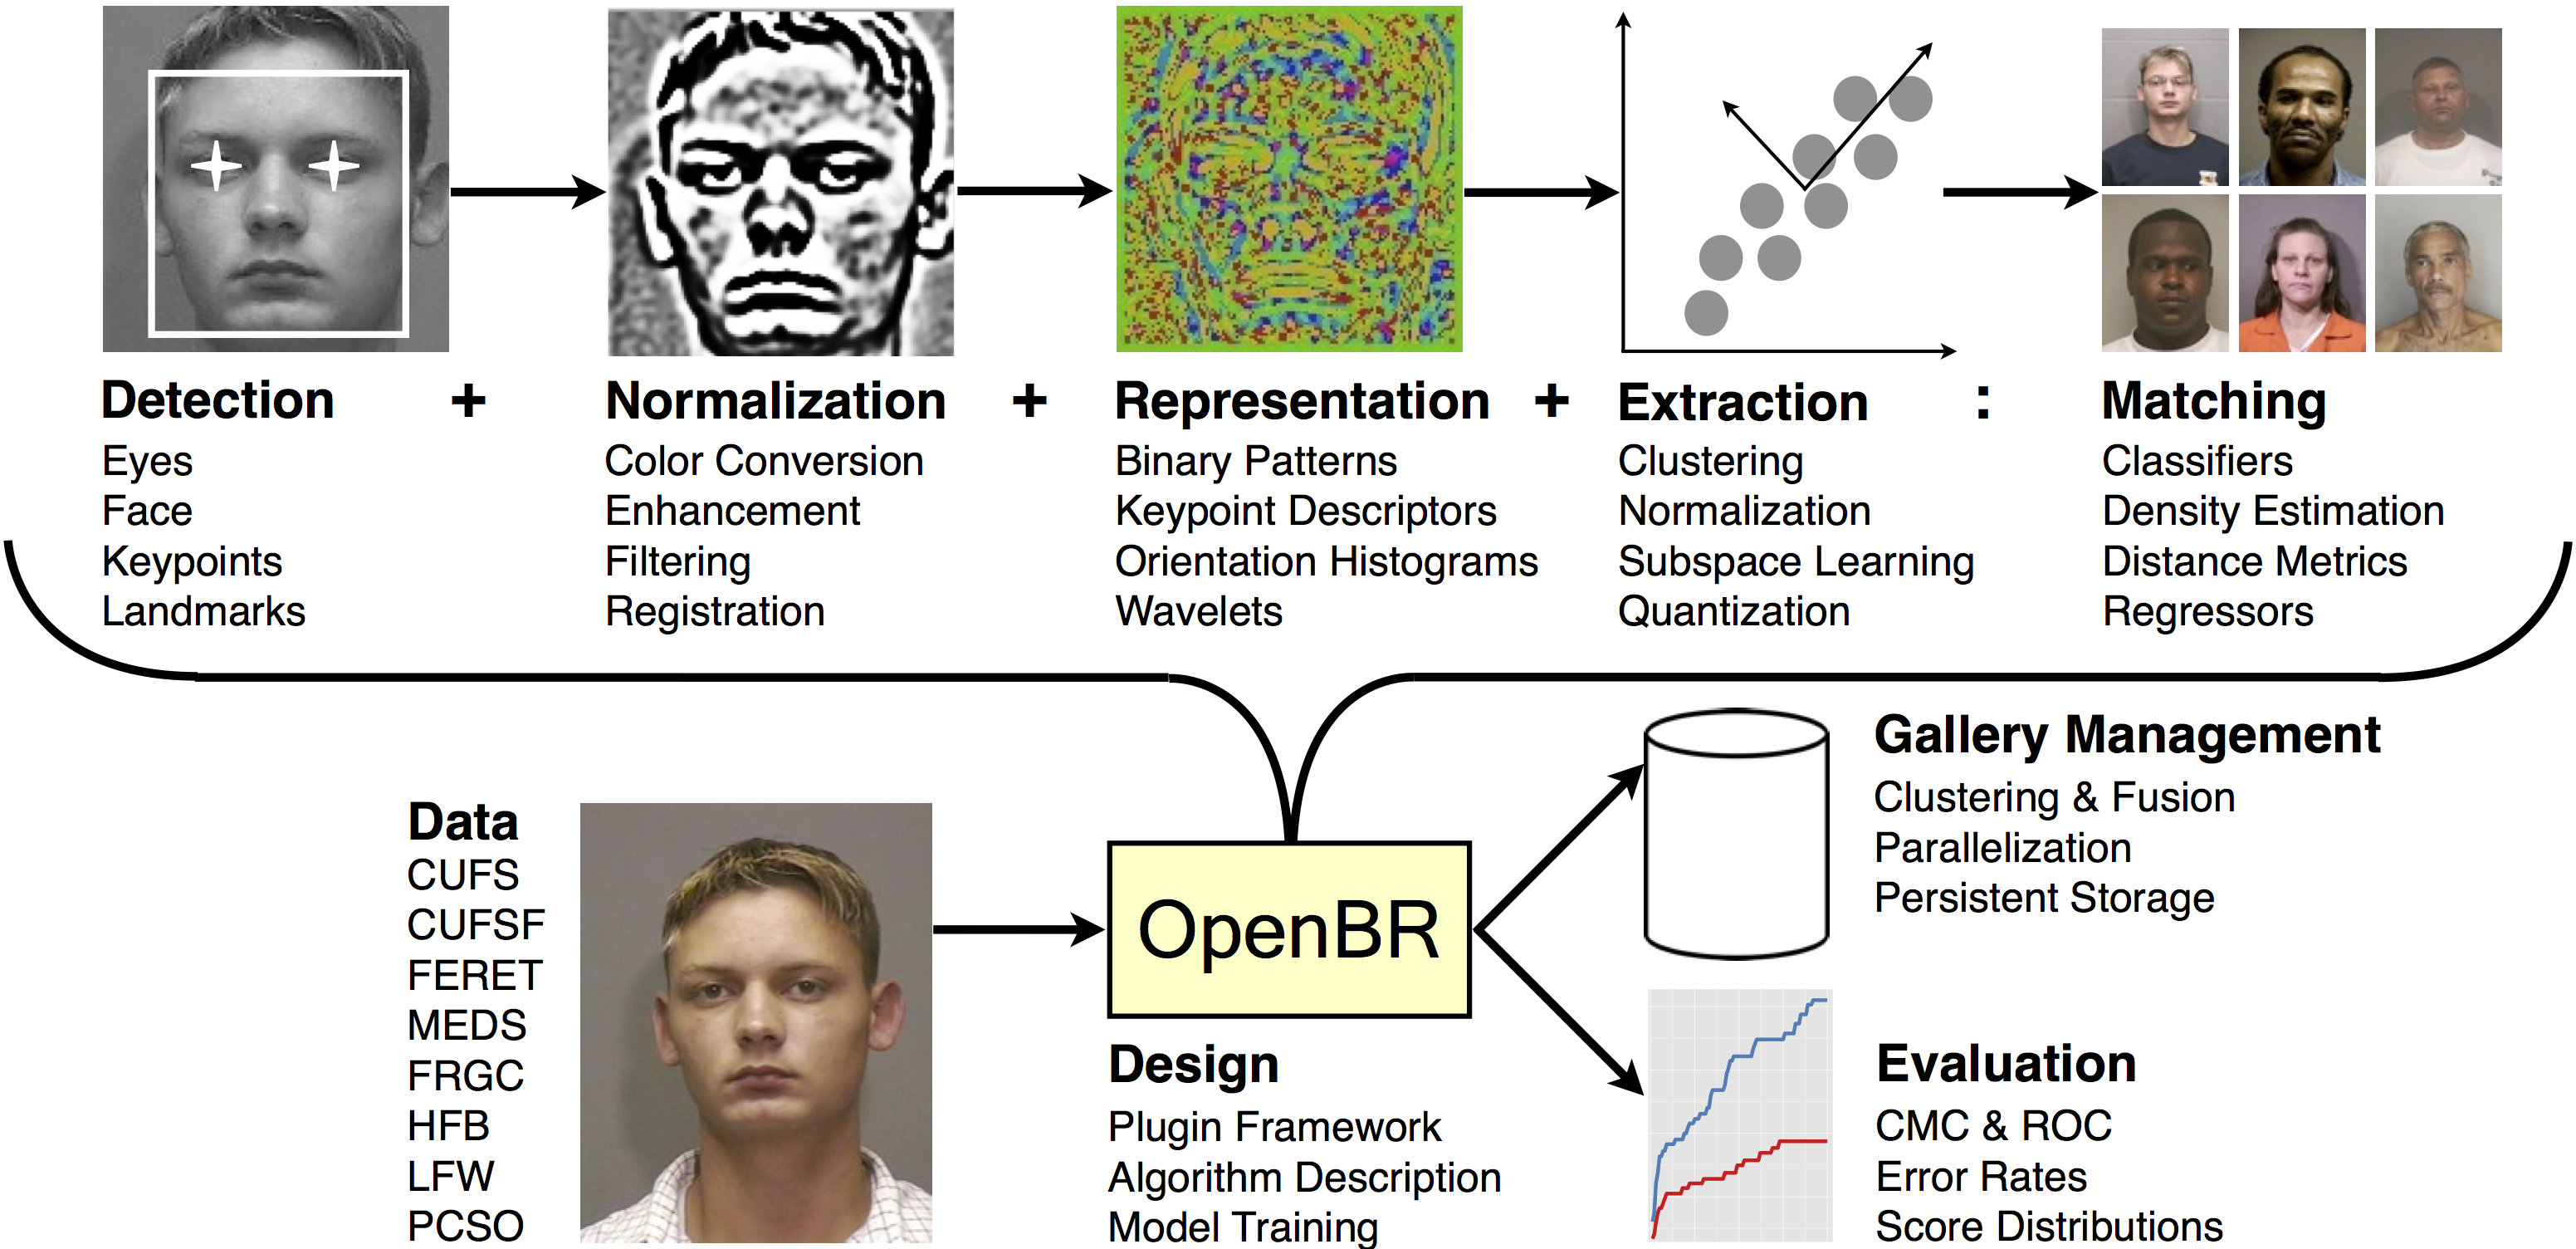
\includegraphics[width=0.7\linewidth]{figures/3-PRMM/OpenBR.png}
	\caption[OpenBR]{Overview of OpenBR Capabilities.}
	\label{fig:2:OpenBR}
\end{figure}

\subsubsection{Magic Mirror concept}
The concept of a MR magic mirror has been proposed to address the challenges in AR related to perception \cite{Grosjean1999}.
A mirror is the most popular way to learn about ourselves. We all spend a lot of time looking in the mirror. It is first thing we look at in the morning to see what we need to do, such as shaving, putting on make-up, and tooth-brushing. We also use it to check if we should go on a diet and figure out what to wear. 
The magic mirror is a user interface technique that mimics a normal mirror and presents non-physical visual feedback in addition to the normally optical effect. Here the user stands in front of a screen and via a camera, the image of the user is shown on the screen such that it acts like a mirror.

The concept of a MR magic mirror has been shown previously, mainly for advertisement and marketing. 
Previous systems augmented onto the user virtual shoes \cite{Eisert2008,Luh2013}, shirts \cite{Ehara2006} and knight's armors \cite{Fiala2007}. For tracking the position of the user, previous systems have used tracking markers or a tracking shirt with a rectangular highly textured region \cite{Hilsmann2008}. For shoes, a vision-based approach has been presented \cite{Eisert2008}.
Based on the tracking technologies of Kinect, Bodymetrics\footnote{\url{http://www.bodymetrics.com/}} created a system in which a 3D avatar is generated for each user whose body shape and size are measured with Kinect. The user can control the 3D avatar through Kinect and see how the virtual clothes look on the avatar in different poses. Fitnect\footnote{\url{http://www.fitnect.com/}} also provides a system for users to try on different clothes, but instead of using an avatar, the virtual clothes are directly displayed on the user's body in augmented videos. Facecake\footnote{\url{http://www.facecake.com/swivel/}} gives a similar augmented reality system called Swivel in which users can virtually try on a variety of fashion products including handbags, clothes, necklace and sunglasses.

All the medical knowledge is about ourselves, but we cannot look through our cloth and skin to directly observe what is inside of the human body. 
While a magic mirror system restricts the motion of the user, it would allow an inexpensive and robust solution for medical education and training. \citet{Blum2012a} presented a magic mirror for teaching anatomy. The system uses a depth camera to track the pose of a user standing in front of a large display. A volume visualization of a CT dataset is augmented onto the user, creating the illusion that the user can look into his/her body.

\subsection{Medical AR Applications}
Many commercially available systems use virtual reality (VR) for medical education and psychomotor skills training. These systems have indeed proven to be valid and are of use in clinical training and teaching \cite{Lewis2011,Thijssen2010,VanDongen2011}. In addition to the advantages of VR, AR systems also have the advantage that information can be embedded and/or superimposed upon reality. This allows for a more close-to-reality presentation of medical knowledge and offers opportunities for more interactive learning and training. The user can also spatially relate virtual objects to the reality. 

\subsubsection{Education}
The General Medical Council recently proposed standards for effective teaching and learning of medical students \cite{Council2009}. They stated that: ``...medical schools should take advantage of new technologies … to deliver teaching.'' 
Augmented reality research has matured to a level that its applications can now be found in both mobile and non-mobile devices \cite{Bacca2014} and research on AR has also demonstrated its extreme usefulness for increasing student motivation in the learning process \cite{Chang2014,DiSerio2013}.

In medical, an AR system for patient-doctor communication has recently been presented \cite{Ni2011}. This system used a hand-held projector to project anatomy onto the skin of the patient. While this system is relatively inexpensive, it could only display anatomy which is close to the skin in correct perspective. Furthermore, it did not automatically track the position of the projector and the patient. The doctor must then figure out manually how to position the projector and the patient in such a way that the anatomy is augmented correctly.

Understanding human anatomy is essential for practicing medicine since anatomical knowledge supports the formulation of a diagnosis and communication of that diagnosis to patient and colleagues \cite{Frank2005}.  AR technology could offer an additional teaching method for anatomy education, depending on how it is implemented. Strong points are the visualization capabilities including the 3D rendering of anatomical imagery.
By combining computer models of anatomical structures with custom software we can showcase to students new ways of interacting with anatomy that could not be achieved during cadaveric dissections or in static images and diagrams for increasing their learning satisfaction \cite{Bacca2014,ma2013ismar,NMC2014}.
Augmented reality systems for visualization of anatomy have been shown before. \cite{Davis2002} presented a system that augmented a 3D model of anatomical airways onto a patient phantom using a head mounted display (HMD). Another system that used a HMD to visualize human anatomy onto a phantom has been shown by \cite{Juan2008a}. Their system allows students to open the abdomen of the phantom and visualizes different organs on the phantom.
Other sensory experiences could be implemented as well, such as tactile feedback. AR provides real-time manipulation of these visualizations and direct feedback to students. With that, AR technology could comply with some affordances of traditional dissection classes. Several AR systems have already been developed specifically for anatomy education \cite{Thomas2010,Chien2010,Blum2012b}. 
\citet{Blum2012b} described `Mirracle' which was an AR system that can be used for undergraduate anatomy education. The set-up of that system is as follows. The trainee stands in front of a TV screen that has a camera and the Kinect attached to it. The camera image of the trainee is flipped horizontally and is shown on the TV screen, mimicking a mirror function. Part of an anonymous patient CT dataset is augmented on the user's body and shown on the TV screen. This creates the illusion that the trainee can look inside their body. 

\subsubsection{Training}
A gesture-based user interface allows real-time manipulation and visualization of the CT data. The trainee can scroll through the dataset in sagittal, transverse and coronal slice mode, by using different hand gestures \cite{Kamphuis2014}.
Consistent with modern learning theories advocating for active participation with immediate application of knowledge \cite{Ponce2014}, virtual interactive presence (VIP) technology enables learners to immerse themselves in a real surgical environment. 
The free-form feedback from the participants in a study organized by \citet{Ponce2014} highlights the potential for an improved educational experience through greater involvement of a resident surgeon. Resident surgeons expressed greater comfort with having the attending surgeon outside the operative room because they experienced a feeling of autonomy while still having sufficient oversight. The attending surgeon commented that instruction was improved since virtually ``touching'' anatomy helped to better communicate degrees of motion. The use of the system to convey hand gestures or point to a particular anatomy was thought to be more effective. Both the resident and attending surgeons thought that the identification of anatomy was better with use of this technology. This pilot study revealed that the VIP technology was efficient, safe, and effective as a teaching tool. The attending and resident surgeons agreed that training was enhanced, and this occurred without increasing operative times. Furthermore, the attending surgeon believed that this technology improved teaching effectiveness \cite{Ponce2014}.

\subsubsection{Real-time navigation}
Surgeons have welcomed AR to assist them only in specific work-flow tasks and in surgical planning. Consequently, it was discussed that augmented reality is a promising solution to improve the accuracy of surgical procedures, decrease the variability of surgical outcomes, reduce trauma to the critical anatomical structures, increase the reproducibility of a surgeons' performance, and reduce radiation exposure \cite{Navab2012a}. 
Medical augmented reality has been successfully applied in various disciplines of surgery, such as neurosurgery, orthopaedic surgery, and maxillofacial surgery \cite{Fallavollita2016}.
\citet{Navab2010} extended a standard mobile C-arm fluoroscope by a video camera and mirror construction, delivering an intuitive real-time intra-operative visualization of X-ray images co-registered with live video.
\citet{Stetten2005} presented a Real-Time Tomographic Reflection (RTTR) as an image guidance technique for needle biopsy. RTTR is a new method of in-situ visualization, which merges the visual outer surface of a patient with a simultaneous ultrasound scan of the patient’s interior using a half-silvered mirror. The ultrasound image is visually merged with the patient, along with the operator's hands and the invasive tool in the operator’s natural field of view. 
\citet{Fichtinger2005} proposed an intraoperative CT-based medical AR system for visualizing one CT slice onto the patient in-situ using a specific arrangement of a half transparent mirror and a monitor rigidly attached to a CT scanner.  
\citet{Feuerstein2008} augmented laparoscopic video images with intraoperative 3D cone-beam CT by tracking both C-arm and laparoscope using the same external optical tracking system. 
%\citet{Wendler2007} fuses real-time ultrasound images with synchronized real-time functional nuclear information from a gamma probe based on optical tracking the ultrasound and nuclear probes in a common coordinate system. 
\citet{Wendler2007a} proposed freehand SPECT to augment the 3D reconstruction of radioactive distributions via live video by using a calibrated optical tracking and video camera system.  
In general, AR has not been widely accepted in clinical practice due to its cumbersome system setups, the requirement of a line-of-sight for tracking, on-site calibration, and a lack of real-time accurate registration between medical data, patient and surgical instruments. Additionally, real-time non-rigid registration methods, display techniques and user-interfaces must be addressed and delivered for surgeon acceptance inside the operating room.

%\paragraph{AR solutions for perception of medical information}
%Some augmented reality applications use polygonal models to augment a real scene. However, most of the medical applications have volumetric data to be visualized. Therefore, it is desirable for the medical AR systems to provide the visualization of these volumes into the real scene in real-time. 
%\citet{Macedo2014} introduced a real-time semi-automatic approach for on-patient medical volume data visualization. This solution is possible in a marker-less augmented reality (MAR) environment, whereas the medical data consists of a volume reconstructed from 3D computed tomography (CT) image data. A 3D reference model of the region of interest in the patient is generated and tracked from a Kinect depth stream. From the estimated camera pose, volumetric medical data can be displayed inside the patient's anatomy at the location of the real anatomy. The authors evaluated the use of standard volume rendering techniques in the context of a MAR environment and demonstrated that these techniques can be applied in this scenario in real-time. 
%In another work, \citet{Macedo2014a} introduced an on-patient focus + context medical data visualization based on volume clipping. From the estimated camera pose, the volumetric medical data can be displayed inside the patient's anatomy at the location of the real anatomy. To improve the visual quality of the final scene, three methods based on volume clipping are proposed to allow new focus + context visualizations. Moreover, the whole solution supports occlusion handling. From the evaluation of the proposed techniques, the results demonstrate that these methods improve the visual quality of the final rendering. 
%\citet{Dixon2013} assess whether perceptual blindness is significant in a surgical context and evaluate the impact of on-screen navigational cuing with augmented reality. Surgeons and trainees performed an endoscopic navigation exercise on a cadaveric specimen. The subjects were randomized to either a standard endoscopic view (control) or an AR view consisting of an endoscopic video fused with anatomic contours. Two unexpected findings were presented in close proximity to the target point: one critical complication and one foreign body (i.e. a screw). Task completion time, accuracy, and recognition of findings were recorded. Authors demonstrated that perceptual blindness was evident in both groups. Although more accurate, the AR group was less likely to identify unexpected findings clearly within view. Advanced navigational displays may increase precision, but strategies to mitigate perceptual costs need further investigation to allow safe implementation.
%\citet{Blum2012b} describes first steps towards a Superman-like X-ray vision where a brain-computer interface (BCI) device and a gaze-tracker are used to allow the user to control the augmented reality (AR) visualization. A BCI device is integrated into two medical AR systems. To assess the potential of this technology feedback from medical clinicians was gathered. While in their pilot study only electromyographic signals are used, the clinicians provided very positive feedback on the use of BCI for medical AR.
\subsection{Collaborative mixed reality}
The world is becoming more complex, so problem solving often needs a team of experts working together. To do this effectively there is a need for collaborative tools.
MR technology allows users to view and interact in real time with both physical objects and virtual information seamlessly, hence MR systems can also be used to create unique collaborative experience. 
MR is ideal for collaborative interfaces to develop radically new types of collaborative experiences. MR technologies could be used to merge the shared perceived realities of different users, as well as enrich each user's own individual experience in collaborative work \cite{Lukosch2015a}. 
For example, 3D virtual information is shared and operated by co-located users, or remote assistance is implemented by annotating the live video of the remote worker. The main objective is to augment the face-to-face collaborative experience and enable remote users to have a feel that they are co-located \cite{Lukosch2015}. 

Several studies have explored the effectiveness of using MR for complex tasks. For example, MR has been shown to improve the effectiveness of individual manual assembly tasks \cite{Baird1999} and the performance time and mental effort in collaborative design tasks \cite{Wang2011}. 
There are many examples of collaborative MR applications. The Studierstube system \cite{Szalavri1998} targeted face-to-face presentations and allowed users to walk around virtual 3D scientific data. \citet{Hollerer1999} enabled indoor AR users to visualize the locations and paths of outdoor AR users, and all users to create shared annotations.
Research on using MR for collaboration among crime scene investigators indicated that using shared visual feedback promoted mutual understanding, led to consensus, and supported hypothesis testing \cite{Poelman2012}. 
\citet{Datcu2014} presented an AR system and the results showed that MR environment could successfully support information exchange in teams operating in the security domain.
\citet{Gauglitz2014} introduced a tablet-based system that incorporates a touchscreen interface through which a remote user could navigate a physical environment and create world-aligned annotations for supporting remote maintenance (see \figurename{\ref{fig:2-bg:drawingsandvirtualnavigation}}). 
\begin{figure}
	\centering
	\includegraphics[width=0.8\linewidth]{"figures/2-bg/drawings and virtual navigation"}
	\caption{In touch with the remote world. A remote user points out an element in the environment (here: a car's engine bay) by drawing an outline around it. The annotation is world-stabilized and displayed in augmented reality to the local user (bottom left), who is holding a tablet.}
	\label{fig:2-bg:drawingsandvirtualnavigation}
\end{figure}
In summary, MR technology is becoming mature enough to support a variety of collaboration scenarios. However, there are still a number of open issues that need further research. One major issue is to remove functional seams and cognitive seams for the user during the cooperation.

\subsection{Serious gaming}
The concept of ``serious gaming'' is often used to describe the use of digital gaming technology to address a specific set of learning objectives, or behavioral goals. As such, they often seek to build upon the increasingly pervasive role games play as an entertainment medium to provide an engaging and entertaining way to communicate educational content \cite{Schuller2013a}. 
Using games to teach skills used in real life or to convey knowledge has in the last years become generally known under the term serious gaming. The goal is to teach the player something practical in an entertaining and ``fun'' way.

More and more researchers and educators have made an effort to integrate serious games into classrooms \cite{Connolly2012}. Serious games create an immersible context wherein students are allowed to experience things and repeat experimentation that are unlikely to be realized in their daily lives. It is believed that their use in educational settings can increase the probability of providing students with authentic learning \cite{Cheng2012}. Moreover, it is hoped that the use of such games can improve student learning motivation \cite{Papastergiou2009}, facilitate knowledge acquisition \cite{Miller2011}, increase task engagement \cite{Annetta2009}, and foster specific abilities such as problem solving and collaboration \cite{Sanchez2011} by appropriately visualizing abstract ideas and key principles of given topics in the game environment \cite{Cheng2015}. 
In the context of anatomy education, Arcade\footnote{\url{http://anatomyarcade.com/}} offers a large collection of anatomy-related arcade games. The games range from crosswords and jigsaw puzzles to more sophisticated ideas like ``Poke-A-Muscle'' game where the user has to select the right muscles as quickly as possible. These games are accompanied with educational videos to provide a base knowledge that can be tested in the games. The games certainly are not suitable for educating medical students, but they are a fun way to learn basic human anatomy.
A recently successful game is the Surgeon Simulator 2013\footnote{\url{http://www.surgeonsim.com/}}. Here, players have to perform different surgeries from the viewpoint of the acting surgeon. In a 3D environment where organs and tools behave in a physically believable way, players have to remove various organs to eventually perform a heart transplant. %The most important gameplay mechanic is probably the unconventional input mechanic, making it very hard to successfully perform all necessary tasks. While the focus of this game is not on education but rather general entertainment, the players still implicitly learn positions and shape of the most important organs of the body.
Another free on-line service more tailored towards patient education is Surgery Squad\footnote{\url{http://www.surgerysquad.com/}}. Here, players can perform different types of surgery in the browser. They are guided by a virtual surgeon explaining the medical background to the surgery and every step involved. They interactively learn about the surgical procedure by listening to the instructions the virtual surgeon gives and subsequently performing them, mostly by using mouse clicking or dragging over certain areas. These interactive surgeries have been created to educate patients or other interested people on how the surgeries or other procedures are being performed, with a minimal baseline of anatomical knowledge.

Serious games can also be developed for rehabilitation training in MR environments. The gaming system offers a motivational component to the patients in performing exercises, introducing entertainment or distracting them from the potential pain. 
In addition, the camera sensor can monitor the patient and provide correction hint/feedback using game elements during rehabilitation exercise. It has the potential to be deployed to the patient household and eliminate the frequent visits of patients to rehabilitation clinics.

\section{Natural user interface using gestures}
Natural User Interface (NUI) is an emerging computer interaction methodology which focuses on human abilities such as touch, vision, voice, motion and higher cognitive functions such as expression, perception and recall. 
NUI seeks to harness the power of a much wider breadth of communication modalities which leverage skills people gain through traditional physical interaction. NUI is part of the larger field of Human Computer Interaction (HCI) which is the design and implementation of interactive computing systems that users can interact with. 
The user's formulation of the desired task needs to be articulated in the input-language. The task is phrased in terms of certain psychological attributes that highlight the important features of the domain for the user which, if mapped clearly onto the input language, simplify the articulation of a task. Direct manipulation can also facilitate the articulation \cite{Dix2009}.
The responses of the input are translated to stimuli for the system. Once a state transition has occurred within the system, the execution phase is completed and the evaluation begins by translating the system's responses into stimuli for the output component. Finally, the response from the output is translated to stimuli for the user. 
%\figurename{\ref{fig:2-bg:HCI}} shows a comparison of HCI styles involving human-computer interaction and human-real world interaction \cite{Rekimoto1995}.
%\begin{figure}
%	\centering
%	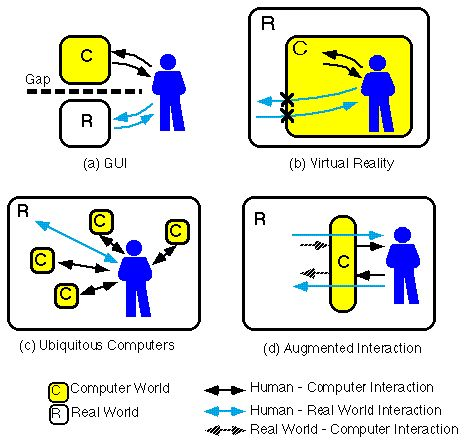
\includegraphics[width=0.6\linewidth]{figures/2-bg/HCI}
%	\caption{ A comparison of HCI styles. (a) In a desk-top computer (with a GUI as its interaction style), interaction between the user and the computer is isolated from the interaction between the user and the real world. There is a gap between the two interactions. Some researchers are trying to bridge this gap by merging a real desk-top with a desk-top in the computer. (b) In a virtual reality system, the computer surrounds the user completely and interaction between the user and the real world vanishes. (c) In the ubiquitous computer environment, the user interacts with the real world but can also interact with computers embodied in the real world. (d) Augmented Interaction supports the user's interaction with the real world, using computer augmented information. }
%	\label{fig:2-bg:HCI}
%\end{figure}

The traditional user interaction consists of the direct manipulation of graphic objects, such as icons and windows, using some type of pointing device. Mouse and keyboard are widely used and well-known for these applications, and recently, users can interact more intuitively using touch-screens. However, the main limitation for these techniques is that the user has to go and grab the device or touch it.  
%requirement for new user interaction method 
It is widely believed that as the computing, communication, and display technologies progress further, the existing user interaction solutions may become a bottleneck for the effective selection and retrieval of desired data. %something about gesture research 
Recognizing gestures for interaction can help achieve the ease and naturalness desired for all human computer interaction. Users generally use hand gestures for expressing their feelings, communicating and notification of their thoughts. The use of hand gestures provides an attractive and natural alternative to some traditional cumbersome devices for human computer interaction. 
%gesture interface
There has been growing interest in the development of new approaches and technologies for bridging the human-computer barrier. Gestures have long been considered as an interaction technique that can potentially deliver more natural, creative and intuitive methods for communicating with our computing devices \cite{Rautaray2015}. 
Gestural interaction is the new excitement in the halls of industry. Advances in the size, power, and cost of microprocessors, memory, cameras, and other sensing devices now make it possible to control by wipes and flicks, hand gestures, and body movements. A new world of interaction is here: The rulebooks and guidelines are being rewritten, or at least, such is the claim. And the new interactions even have a new marketing name: natural, as in ``Natural User Interface''.
Numerous methods for vision-based hand gesture recognition have been developed and evaluated. There are many applications about information processing \cite{Moyle2002,Lenman2002} and visualization as the premier solutions, followed by robotics and sign language \cite{Swindells2002,Osawa2000}. 
Since the release of commercial depth sensors, there have been numerous inspiring successes in finger tracking and hand gesture recognition for human computer interaction \cite{ZhouRen2011,Kulshreshth2013}. \citet{Ruppert2012a} presented a touchless gesture interface which enables the control of a mouse pointer of a computer using \textit{InVesalius}. 

\paragraph{Challenges with normal hand gestures}
Swindell\cite{Swindells2002} indicated an important problem that occurs in many scenarios -`` \textit{the user is aware of where the computing device is but could not directly begin interaction with the device since excess time is lost to build-up connection with the device}". It is known that the geometry of the hand and the mapping from the hand movement to the selected object are hard to reconstruct \cite{Raheja2011}.
In addition, most gestures are neither natural nor easy to learn or remember. Few are innate or readily predisposed to rapid and easy learning. Even the simple head shake is puzzling when cultures intermix. Westerners who travel to India experience difficulty in interpreting the Indian head shake, which at first appears to be a diagonal blend of the Western vertical shake for "yes" and the horizontal shake for "no." Similarly, hand-waving gestures of hello, goodbye, and "come here" are performed differently in different cultures. To see a partial list of the range of gestures used across the world, look up "gestures" and "list of gestures" in Wikipedia.
More important, gestures lack critical clues deemed essential for successful human-computer interaction. Because gestures are ephemeral, they do not leave behind any record of their path, which means that if one makes a gesture and either gets no response or the wrong response, there is little information available to help understand why. The requisite feedback is lacking. Moreover, a pure gestural system makes it difficult to discover the set of possibilities and the precise dynamics of execution. These problems can be overcome, of course, but only by adding conventional interface elements, such as menus, help systems, traces, tutorials, undo operations, and other forms of feedback and guides.

\subsection{Pointing gesture}
%Eye-rooted pointing has been used as a virtual pointer for object selection in virtual environment and pointing and clicking techniques with large displays from a distance.
Pointing gestures are fundamental to human behavior \citep{Matthews2012} and are used consistently across cultures  \citep{McNeill2000}. The gestures begin at an early developmental stage \citep{Carpendale2010} and let humans reference proximal objects as well as abstract concepts in the world. Today, pointing gestures are not only part of our gestural language but are inherently used for interaction \citep{Nanayakkara2013a}. Regarding the ray's origin, pointing techniques can be classified into two groups: \textit{hand-rooted}, where the ray originates at the user's hand, and \textit{eye-rooted}, where the ray starts at the user's eyes. Whenever a \textit{hand-rooted} technique is used, the objects that are along the pointing ray might differ from those that the user focuses on \citep{Argelaguet2008}. The more interesting scenario is the latter.
A number of studies have demonstrated that pointing gestures result in quite effective interactions in virtual environments  \citep{Argelaguet2008} and with very large, high resolution displays \citep{Vogel2005}.

%\textbf{Virtual Pointer} 
\paragraph{Virtual Pointer} The \textit{eye-rooted} pointing technique is developed as a virtual pointer for object selection in virtual environments. The simplest approach, occlusion selection, used a selection ray which was defined as beginning from the user's eye position and pointing to the user's hand position \citep{Forsberg1996,Pierce1997}. \citet{Forsberg1996} defined the origin to be one of the positions of the user's two eyes or an average of them. Alternatively, \citet{Argelaguet2008} proposed a hybrid technique in which the ray started from the user's eye position and its direction was controlled by the hand orientation. All eye positions in these papers was known as it was manually defined during scene rendering.

%\textbf{Distant Pointing} 
\paragraph{Distant Pointing} The \textit{eye-rooted} pointing technique also allows users to perform interaction with a remote display by directly pointing at the object they want to interact with. The remote pointing position is defined by the ray casting from the user's eye to their fingertip.  
\citet*{Liang1994} first presented a highly interactive 3D model by computing a ray going from the user's eye through a hand-held bat while two tracking devices monitored the user's head and the bat. 
\citet{Nickel2003} explored computer vision methods to recognize the body, hand, and finger positions in 2D/3D space to calculate the pointing direction. A vision-based human-computer interaction system was presented by \citet{Reale2011}, integrating components using multiple gestures, including eye gaze, head pose, hand pointing, and mouth motion. 
\citet*{Vogel2005} employed the \textit{Vicon} motion tracking system to analyze the hand-based ray casting and relative pointing with clutching. 
\citet{Banerjee2012} developed \textit{MultiPoint}, a set of perspective-based remote pointing techniques that allowed users to perform remote manipulation of graphical objects on large displays while extra cameras and motion trackers were employed to detect the eye and finger. 
\citet{Huang2014} developed \textit{Dart-it}, a lightweight system that enables perspective-based remote direct-pointing on any remote display using only one RGB-D camera. However, since the recovered pointing ray requires reliable eye and fingertip tracking, all the above methods require external camera or motion trackers for their real-world deployment.

%\textbf{Interaction with an egocentric setup} 
\subsection{Natural interaction in an egocentric setting}
A few authors have tried to estimate the user's eye position and recover the \textit{eye-rooted} pointing geometry to enable interacting with ambient media and objects in the real world. 
One existing technique consists in positioning a camera next to the monitor or on the ceiling to observe the user and implement the outside-in tracking. In this case, the computing device calculates the eye position by detecting the user's gaze and face or wearable trackers. Unfortunately, the user has to stand within a limited working zone defined by the camera, as shown in \figurename{\ref{fig:1-intro:problem}(a)}.
As a solution, authors in  \cite{Mistry2009,Harrison2011} suggest that the camera be kept to a similar view in an egocentric setting.

The interaction between the user and any device can begin with a signal sent using their hands or their eye-gaze estimated within FOV of the wearable camera.

\paragraph{Gesture interaction} Several articles focused on natural gesture interaction methodologies, in which sensors detect and track the pose of the user's arm, hands or fingers to recognize the gesture interaction.
\citet{DeCampos2006} proposed a framework combining a coarse-to-fine method for shape detection and 3D tracking that could identify pointing gestures and estimated their directions in the wearable domain. A gesture recognition algorithm was developed for an interactive museum using 5 different gestures by  \citet{Garcia-Rodriguez2011}. 
\citet{Colaco2013a} presented \textit{Mime}, a compact, low-power 3D sensor for unencumbered free-form, single-handed gestural interaction with HMDs.

\paragraph{Relative pointing} Often a visual feedback is provided to hint where the potential object of interest might be. The user has to learn how to use the natural gesture movement to control the feedback cursor.
\citet{Mistry2009} proposed to bring information out into the tangible world by using a tiny projector and camera mounted on a hat in order to help the user indirectly point to and manipulate the information in the real word.

\paragraph{Natural pointing} Solutions for natural pointing in an egocentric setting in different scenarios have been previously proposed. 
(1) In the case where the object is reachable, the sensor can directly detect which object the user is pointing at without the need for defining a pointing ray and/or its origin.  \textit{OmniTouch} \citep{Harrison2011} is a wearable depth-sensing and projection system that enables interactive multi-touch applications on everyday reachable surfaces.  
SemanticPaint \citep{Valentin2015b} allows users to segment the scene simply by reaching out and touching any desired object or surface. 
(2) \citet{Ha2014} developed a video-see-through augmented reality (AR) system allowing the user to manipulate virtual 3D objects with their bare hand. A bare hand-based interaction with reachable virtual objects in an egocentric viewpoint was also developed by  \citet{Jang2015}.
Here, the user's view was controlled by the computer and the user's eye position was defined during the rendering procedure. Hence, the origin of the pointing ray was manually defined. 
(3) \textit{Pupile} \citep{Kassner2014} provides an accessible, affordable, and extensible open source platform for eye tracking and gaze-based interaction. The eye position is taken as the origin point and the pointing direction is also directly estimated from the eye gaze. 
(4) \citet{ma2015ismar} defined a virtual eye center as the pointing origin after moving the fingertip along the pointing rays. %when interacting with ambient objects. 
The disadvantage of this method is that the user has to keep his/her head still and the calibration procedure is not user friendly. 

Usually the head, eye, hand, and/or finger are detected and tracked to recover the pointing ray. Also, the interaction techniques are implemented using different techniques, for example: (i) with or without visual feedback, (ii) based on direct or relative positioning, (iii) acting on dynamic or static scene, (iv) {functioning} within reachable or unreachable objects in the work space, and (v) extended in the real world or only within the virtual world. 
\tablename{ \ref{tb:relatedWork}} summarizes the characteristics of the above-mentioned methods based on the objects to detect and track and the properties of the interaction techniques. 
% !TEX root = ../thesis-example.tex
%\newgeometry{margin=1cm} % modify this if you need even more space
%\begin{landscape}
\begin{sidewaystable}
	\caption{The objects to track and the properties of the interaction in different works}
	\label{tb:2-bg:pointing}
	\scriptsize
	\centering
	\begin{threeparttable}
		\begin{tabular}{P{5cm}|P{1cm}|P{1cm}|P{1cm}|P{1cm}|P{1cm}|P{1cm}|P{2cm}|P{2cm}|P{2cm}|P{2cm}}
			\hline
			\space & \multicolumn{4}{c}{Objects to Track} & \multicolumn{6}{|c}{Interaction} \\
			\hline
			Work & Head & Eye & Hand & Finger & Visual Feedback & Direct & Dynamic Scene & Unlimited Distance & Real World & Virtual World\\
			%\hline
			\citet{Pierce1997} & \xmark & \xmark \tnote{a}  & \cmark \tnote{b} & \cmark \tnote{b} & \cmark & \cmark & \cmark & \cmark & \xmark & \cmark \\
			\citet{Argelaguet2008} & \xmark & \xmark \tnote{a}  & \cmark & \cmark & \cmark & \cmark & \cmark & \cmark & \xmark & \cmark \\
			\citet{Liang1994} & \xmark & \xmark \tnote{a}  & \cmark\tnote{b} & \cmark\tnote{b} & \cmark & \cmark & \xmark & \cmark & \cmark & \cmark \tnote{c} \\
			\citet{Nickel2003} & \cmark & \cmark  & \cmark & \cmark & \cmark & \cmark & \xmark & \cmark & \cmark & \xmark\\
			\citet{Banerjee2012} & \xmark & \cmark  & \cmark & \cmark & \cmark & \cmark & \xmark & \cmark & \cmark & \xmark\\
			\citet{Huang2014} & \xmark & \cmark  & \xmark & \cmark & \xmark & \cmark & \xmark & \cmark & \cmark & \xmark\\
			\citet{DeCampos2006} & \xmark & \xmark  & \cmark & \cmark & \cmark & \xmark & \cmark & \cmark & \cmark \tnote{d} & \cmark \tnote{d}\\
			\citet{Colaco2013a} & \xmark & \xmark  & \cmark & \cmark & \cmark & \xmark & \cmark & \cmark & \cmark & \cmark\\
			\citet{Mistry2009} & \xmark & \xmark  & \xmark & \cmark & \cmark & \xmark & \cmark & \cmark & \cmark & \xmark\\
			\citet{Harrison2011} & \xmark & \xmark  & \cmark & \cmark & \xmark & \cmark & \cmark & \xmark & \cmark & \xmark\\
			\citet{Ha2014} & \xmark & \xmark \tnote{a}  & \cmark & \cmark & \cmark & \cmark & \cmark & \cmark & \cmark \tnote{e} & \cmark\\
			\citet{Jang2015} & \xmark & \xmark \tnote{a}  & \cmark & \cmark & \cmark & \cmark & \cmark & \xmark & \xmark & \cmark\\
			\citet{Kassner2014} & \xmark & \cmark  & \xmark & \xmark & \cmark & \cmark & \cmark & \cmark & \cmark \tnote{d} & \cmark \tnote{d}\\
			Our method &  \xmark & \xmark \tnote{f} & \xmark & \cmark & \xmark & \cmark & \cmark & \cmark & \cmark \tnote{d} & \cmark \tnote{d}\\
			\end{tabular}
			\begin{tablenotes}
				\item[a] The eye position is defined during rendering procedure.
				\item[b] Special tool is tracked instead of hand and finger.
				\item[c] 3D virtual world is shown in 2D display.
				\item[d] The method could be used in this scenario with proper hardware.
				\item[e] The Real world is shown via video see through HMD.
				\item[f] The eye position is calculated via the tracking of the finger and scenario.
				\end{tablenotes}
				\end{threeparttable}
				\end{sidewaystable}
%\end{landscape}
%\restoregeometry
